\documentclass[a4paper,10pt]{article}
\usepackage{trymtex}
\usepackage[backend=biber,style=alphabetic]{biblatex}
\usetikzlibrary{arrows.meta,calc,positioning}

\addbibresource{references.bib}

\begin{document}
\begin{titlepage}
    \newcommand{\HRule}{\rule{\linewidth}{0.5mm}}
    \begin{tikzpicture}[remember picture, overlay]
      % NTNU logo
      \node[anchor=north west, xshift=1.0cm, yshift=-1.0cm] at (current page.north west) {
        
\includegraphics[width=2.0cm]{figures/ntnu_logo_liten.png}
      };
    \end{tikzpicture}
  
    \center

    % Course code & title
    {\color{ntnu-blue}\sffamily\large TMA4212 \par}
    {\sffamily\Large Numerical Solution of Differential Equations by Difference Methods \par}
    
    \HRule
    \vspace{1.5cm}
  
    % Assignment title
    {\large\sffamily\bfseries Project 2\par}
    \vspace{0.3cm}
    {\Large\sffamily\textit{Solving the Poisson equation, and an Optimal Control Problem\\ using the Finite Element Method}\par}
  
    \vspace{0.5cm}
    \HRule
  
    \vfill
  
    % Author info
    \begin{minipage}{0.6\textwidth}
      \begin{flushleft}
        \large
        \textbf{Authors:}\\
        Haugen, Tor Ludvig Løvold \\
        Sæther, Trym\\ 
      \end{flushleft}
    \end{minipage}%
    \begin{minipage}{0.4\textwidth}
      \begin{flushright}
        \large
        \textbf{Semester:}\\
        Spring 2025
      \end{flushright}
    \end{minipage}
  
    % University logo/name
    \begin{center}
      {\color{ntnu-blue}\sffamily\Large Norwegian University of Science and Technology}\\
      \vspace{0.3cm}
      {\sffamily\large Department of Mathematical Sciences}
  
      \vspace{0.5cm}
      {\large\today}
    \end{center}
  
    \vspace{1cm}
  \end{titlepage}
  
  
  
\clearpage

\section{Solving a 1D Poisson Equation with Quadratic Finite Elements}

\subsection{Problem Statement and Variational Formulation}

We consider the one-dimensional Poisson equation
\[
	-u''(x)=f(x), \quad x\in\Omega=(0,1),
\]
with homogeneous Dirichlet boundary conditions \(u(0)=u(1)=0\).
To solve this boundary value problem using the finite element method, we first derive its \emph{variational (weak) form}. We seek \(u\in H_0^1(\Omega)\) such that for all test functions \(v\in H_0^1(\Omega)\) the following holds:
\[
	a(u,v)=F(v),
\]
where the bilinear form and linear functional are given by
\[
	a(u,v)=\int_0^1 u'(x)v'(x)\,dx,\qquad F(v)=\int_0^1 f(x)v(x)\,dx.
\]
This weak formulation is obtained by multiplying the differential equation by \(v\), integrating over \(\Omega\), and performing integration by parts (with the boundary terms vanishing due to \(v(0)=v(1)=0\)). The Lax--Milgram theorem guarantees the existence of a unique solution \(u\in H_0^1(\Omega)\) for each \(f\in L^2(\Omega)\).

In the Galerkin finite element method the infinite-dimensional problem is restricted to a finite-dimensional subspace \(V_h\subset H_0^1(\Omega)\). We choose \(V_h\) to be the space of \emph{continuous piecewise-quadratic \(\mathbb{P}_2\) polynomials} on a partition of \(\Omega\). In other words, the discrete problem is: find \(u_h\in V_h\) such that
\[
	a(u_h,v_h)=F(v_h)\quad\forall\, v_h\in V_h.
\]
This formulation leads to a linear system for the coefficients of \(u_h\) in a finite element basis.

\subsection{Quadratic Finite Element Discretization (\(\mathbb{P}_2\) Lagrange Elements)}

\paragraph{Mesh and basis functions}
Let \(0=x_0<x_2<\cdots<x_{2N}\) be a partition of \([0,1]\) into \(N\) elements \(K_i=(x_{2i},x_{2i+2})\) with variable element lengths \(h_i=x_{2i+2}-x_{2i}\).
On each element we approximate \(u(x)\) by a quadratic polynomial.
Globally, the finite element space is defined by

\[
	V_h=\{v\in C^0([0,1])\;:\; v|_{K_i}\ \text{is a polynomial of degree}\le2,\quad\forall i\},
\]

together with the condition \(v(0)=v(1)=0\) (homogeneous Dirichlet conditions).
This describes the \emph{\(\mathbb{P}_2\) Lagrange finite element space}.
For a mesh with, say, 5 elements (yielding 6 nodes) and 5 midpoints, the total number of potential basis functions is \(11\);
however, since the two boundary nodes are prescribed, there are \(2N-1\) unknowns.

Each quadratic element has three local degrees of freedom (DoFs): the two endpoints and the midpoint.
On a reference element
\[
	\hat{K}=[0,1]
\]
with reference nodes \(\hat{\xi}_i=\{0,\tfrac{1}{2},1\}\) we define the Lagrange shape functions \(\{\Psi_0(\xi),\Psi_1(\xi),\Psi_2(\xi)\}\subset \mathbb{P}_2(\hat{K})\) such that
\[
	\Psi_\alpha(\hat{\xi}_\beta)=\delta_{\alpha\beta}.
\]
By Lagrange interpolation one obtains:
\[
	\Psi_0(\xi)=2\xi^2-3\xi+1,\qquad \Psi_1(\xi)=-4\xi^2+4\xi,\qquad \Psi_2(\xi)=2\xi^2-\xi.
\]
On any physical element \(K_i=(x_{2i},x_{2i+2})\), the mapping is given by the affine transformation
\[
	\Phi_{K_i}:\hat{K}\to K_i,\quad x=\Phi_{K_i}(\xi)=x_i+\xi\,h_i,
\]
so the physical shape functions are defined as
\[
	\phi_\alpha^{(i)}(x)=\Psi_\alpha(\xi),\quad \text{with } \xi=\frac{x-x_i}{h_i}.
\]
Globally, the finite element function \(u_h(x)\) is expanded in terms of basis functions \(\{\varphi_j(x)\}\):
\[
	u_h(x)=\sum_{j=1}^{2N-1} u_j\,\varphi_j(x),
\]
where \(U_j\) are the unknown coefficients corresponding to interior nodes and midpoints. Substituting this expansion into the weak formulation using \(v_h=\varphi_i\) leads to the linear system
\[
	AU=F,
\]
with entries
\[
	A_{ij}=\int_0^1\varphi_j'(x)\varphi_i'(x)\,dx,\qquad F_i=\int_0^1 f(x)\varphi_i(x)\,dx.
\]

\subsection{Discrete Galerkin Formulation: Local Stiffness Matrix and Load Vector}

On each element \(K_i=(x_i,x_{i+1})\) with local basis functions \(\phi_0^{(i)},\phi_1^{(i)},\phi_2^{(i)}\), the element stiffness matrix is defined as
\[
	A^{(i)}_{\alpha\beta}=\int_{x_i}^{x_{i+1}} \big(\phi_\beta^{(i)}\big)'(x) \big(\phi_\alpha^{(i)}\big)'(x)\,dx,
\]
and the element load vector as
\[
	F^{(i)}_\alpha=\int_{x_i}^{x_{i+1}} f(x)\,\phi_\alpha^{(i)}(x)\,dx.
\]

\textbf{Local stiffness matrix:} With the affine mapping \(x=x_i+\xi\,h_i\) (so that \(dx=h_i\,d\xi\)) and
\[
	\frac{d\phi_\alpha^{(i)}}{dx}=\frac{1}{h_i}\Psi_\alpha'(\xi),
\]
the stiffness matrix becomes
\[
	A^{(i)}_{\alpha\beta}=\frac{1}{h_i}\int_0^1 \Psi_\alpha'(\xi)\Psi_\beta'(\xi)\,d\xi.
\]
The reference integral
\[
	\int_0^1 \Psi_\alpha'(\xi)\Psi_\beta'(\xi)\,d\xi
\]
is the same for all elements. With
\[
	\Psi_0'(\xi)=4\xi-3,\quad \Psi_1'(\xi)=-8\xi+4,\quad \Psi_2'(\xi)=4\xi-1,
\]
one finds
\[
	\int_0^1 \Psi_\alpha'(\xi)\Psi_\beta'(\xi)\,d\xi = \frac{1}{3}
	\begin{pmatrix}
		7  & -8 & 1  \\[1mm]
		-8 & 16 & -8 \\[1mm]
		1  & -8 & 7
	\end{pmatrix}_{\alpha\beta}
\]
Thus, the local stiffness matrix on element \(K_i\) is
\[
	A^{(i)}=\frac{1}{h_i}\,\frac{1}{3}
	\begin{bmatrix}
		7  & -8 & 1  \\[1mm]
		-8 & 16 & -8 \\[1mm]
		1  & -8 & 7
	\end{bmatrix}.
\]

\paragraph{Local load vector}
For the load vector on \(K_i\) we have:
\[
	F^{(i)}_\alpha=h_i\int_0^1 f(x_i+\xi h_i)\,\Psi_\alpha(\xi)\,d\xi.
\]
Using Simpson's rule over \([0,1]\) (with nodes \(\xi=0,0.5,1\)) gives:
\[
	\int_0^1 g(\xi)d\xi\approx \frac{1}{6}\Big[g(0)+4g(0.5)+g(1)\Big].
\]
Since \(\Psi_\alpha(\xi_\beta)=\delta_{\alpha\beta}\), we deduce:
\[
	F^{(i)}_0\approx \frac{h_i}{6}f(x_i),\quad
	F^{(i)}_1\approx \frac{2h_i}{3}f\!\left(\frac{x_i+x_{i+1}}{2}\right),\quad
	F^{(i)}_2\approx \frac{h_i}{6}f(x_{i+1}).
\]

\paragraph{Assembly and global system}
Using a local-to-global mapping \(\theta(i,\alpha)\) that assigns a global index to each local node on element \(K_i\):
\[
	\theta(i,0) = \text{index of node at } x_i,\quad
	\theta(i,1) = \text{index of midpoint } \left(\frac{x_i+x_{i+1}}{2}\right),\quad
	\theta(i,2) = \text{index of node at } x_{i+1},
\]
the local matrices and load vectors are assembled into the global stiffness matrix \(K\) and load vector \(F\). (Contributions involving boundary nodes are omitted since \(u(0)\) and \(u(1)\) are prescribed.) This yields a symmetric positive-definite system
\[
	KU=F,
\]
of size \((2N-1)\times(2N-1)\).

\subsection{Verification of Local Formulas}

For a uniform mesh (\(h_i=h\)) the assembled system exhibits the standard 5-point stencil for a one-dimensional second-order problem.

\begin{figure}[H]
	\centering
	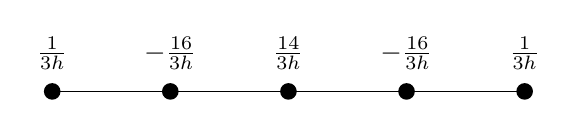
\begin{tikzpicture}[scale=1.5]
		% Dots
		\foreach \x in {-2,-1,0,1,2} {
				\fill (\x,0) circle (2pt);
			}

		% Labels for weights
		\node[above] at (-2,0.1) {\(\frac{1}{3h}\)};
		\node[above] at (-1,0.1) {\(-\frac{16}{3h}\)};
		\node[above] at (0,0.1) {\(\frac{14}{3h}\)};
		\node[above] at (1,0.1) {\(-\frac{16}{3h}\)};
		\node[above] at (2,0.1) {\(\frac{1}{3h}\)};

		% Connecting lines
		\draw (-2,0) -- (2,0);
	\end{tikzpicture}
	\caption{Stiffness matrix pattern for uniform mesh}
\end{figure}


For example, an interior node appears in two element matrices, summing to a row with pattern
\[
	\Bigl(\dots,\frac{1}{3h}, -\frac{16}{3h}, \frac{14}{3h}, -\frac{16}{3h}, \frac{1}{3h},\dots\Bigr)
\]
which corresponds to a second-order accurate discretization of \(-u''\). Similarly, the load vector obtained by approximating \(\int_0^1 f\varphi_i\) matches the Simpson rule based weights.

\subsection{Implementation and Numerical Results}

The \(\mathbb{P}_2\) finite element solver was implemented in Python. The code constructs the mesh and the mapping of local to global degrees of freedom, computes the element stiffness matrices and load vectors using Simpson's rule, assembles the global system, and solves it with a dense linear solver. This implementation naturally accommodates non-uniform meshes by computing the individual element lengths \(h_i\) and applying the corresponding formulas.

For instance, when solving
\[
	-f''(x)=\pi^2\sin(\pi x),\qquad u(x)=\sin(\pi x),
\]
on \([0,1]\) with \(u(0)=u(1)=0\), a uniform mesh with \(N=4\) elements (each \(h=0.25\)) produces a finite element solution \(u_h(x)\) that nearly coincides with the exact solution. Figure~2 shows a plot of \(u_h\) (orange solid line) against \(u\) (black dashed line), where the maximum error is of order \(10^{-3}\).
\begin{figure}[H]
	\centering
	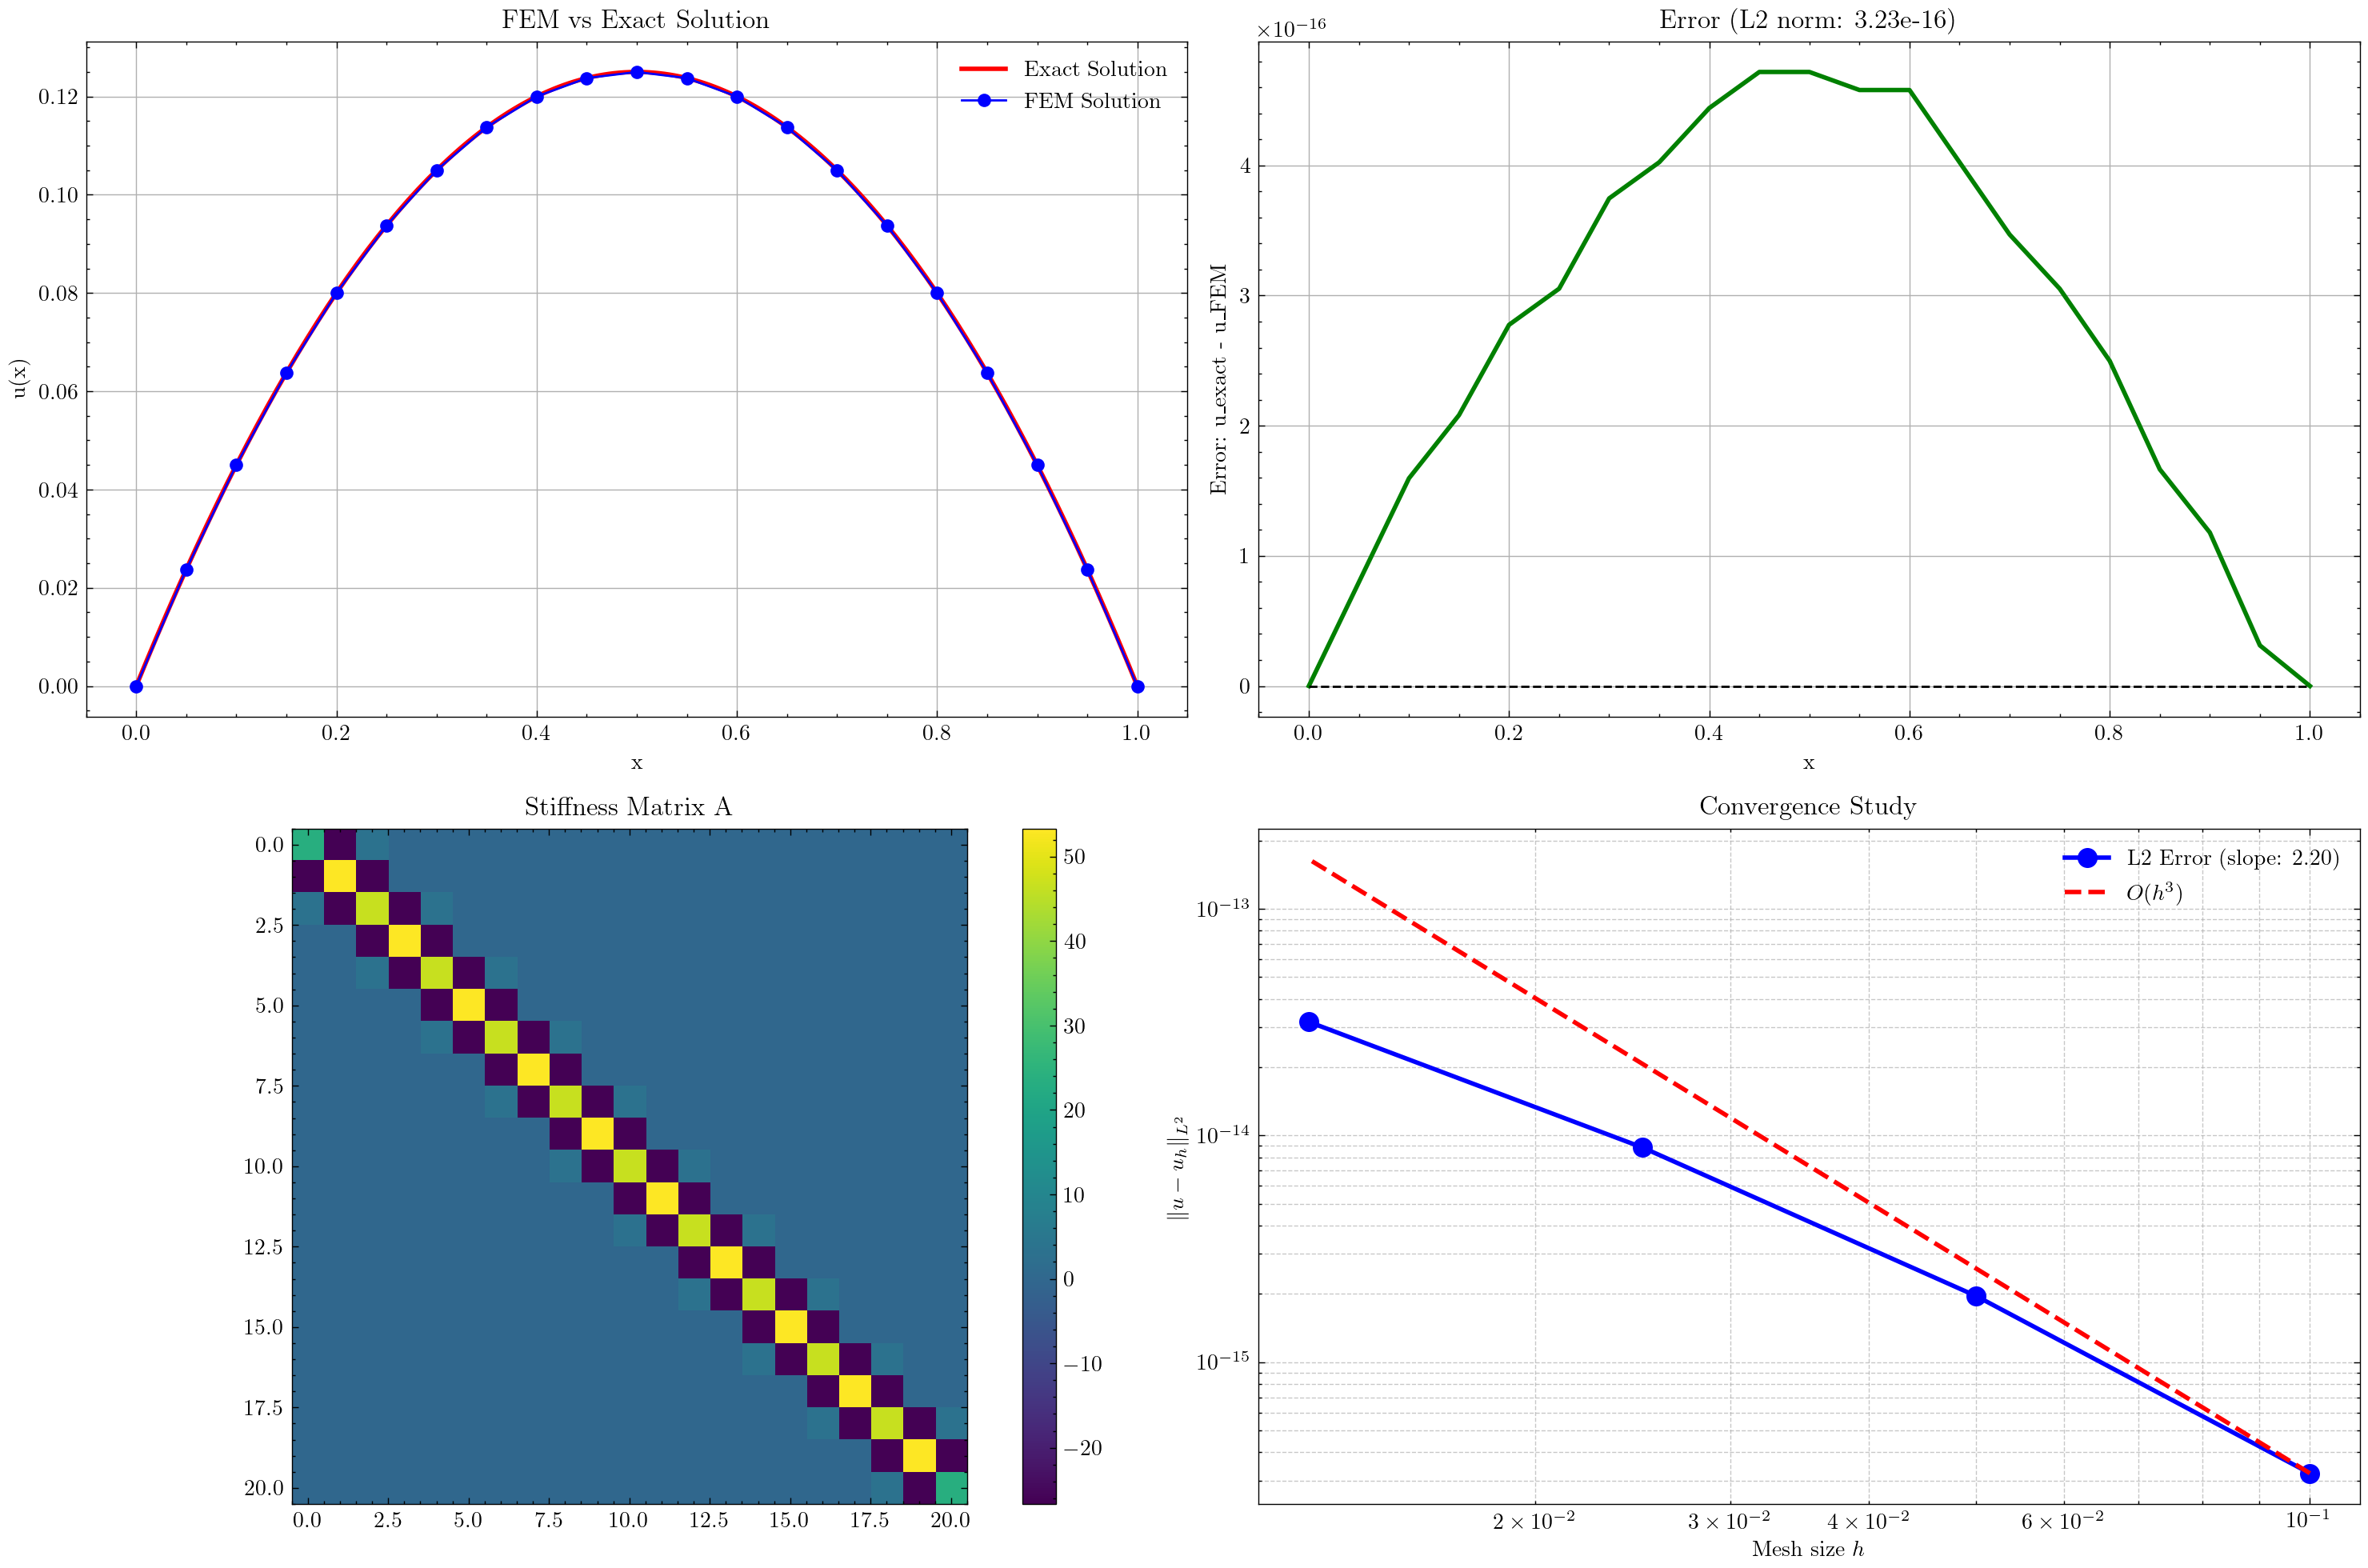
\includegraphics[width=0.8\textwidth]{figures/poisson_1.png}
	\caption{Comparison of exact solution \(u(x)\) (dashed line) and finite element solution \(u_h(x)\) (solid line), \(\mathrm{L}_2\) error plot, Stiffness matrix pattern and \(\mathrm{L}_2\) convergence plot against \(\mathcal{O}(h^3)\) for the Poisson problem with \(N=4\) elements.}
\end{figure}

To quantify the error, the \(L^2\)-norm of the error
\[
	\|e\|_{L^2} = \sqrt{\int_0^1 |u(x)-u_h(x)|^2\,dx}
\]
was computed using a composite Simpson rule on a fine grid. Table~1 summarizes the error for various mesh refinements. As the mesh is refined, halving \(h\) reduces the \(L^2\) error by approximately a factor of 8, confirming the third-order accuracy (\(O(h^3)\)) of the quadratic finite element method in the \(L^2\) norm. In contrast, linear elements (P1) exhibit second-order convergence.

Thus, both theoretical error analysis and numerical experiments demonstrate that the quadratic finite element method is highly accurate for the given Poisson problem.
\begin{minted}[linenos,frame=lines]{python}
import numpy as np

def f(x):
    return np.pi**2 * np.sin(np.pi*x)

# Define mesh (example: non-uniform points or uniform linspace)
x_nodes = np.array([0, 0.2, 0.5, 0.7, 1.0])  # example non-uniform mesh
N = len(x_nodes) - 1

# Assign global indices for interior node and midpoint DoFs
node_index = [-1] * (N + 1)
mid_index = [None] * N
glob_idx = 0
for j in range(1, N):       # interior nodes
    node_index[j] = glob_idx
    glob_idx += 1
for i in range(N):          # midpoints
    mid_index[i] = glob_idx
    glob_idx += 1

# Initialize global stiffness matrix K and load vector F
size = glob_idx
K = np.zeros((size, size))
F = np.zeros(size)

# Assemble the global stiffness matrix and load vector
psi_vals = {0: np.array([1, 0, 0]),
            0.5: np.array([0, 1, 0]),
            1: np.array([0, 0, 1])}
psi_prime = {0: np.array([-3, 4, -1]),
             0.5: np.array([-1, 0, 1]),
             1: np.array([1, -4, 3])}

for i in range(N):
    h_i = x_nodes[i+1] - x_nodes[i]
    # Element stiffness via Simpson's rule on reference [0,1]:
    for a in range(3):
        for b in range(3):
            # Simpson's rule with reference shape function derivatives
            val0 = psi_prime[0][a] * psi_prime[0][b]
            valm = psi_prime[0.5][a] * psi_prime[0.5][b]
            val1 = psi_prime[1][a] * psi_prime[1][b]
            K_elem = (val0 + 4*valm + val1) * (1 / (6 * h_i))  # 1/h  (1/6)[...]
            # Map local (a, b) to global indices
            p = node_index[i] if a == 0 else (mid_index[i] if a == 1 else node_index[i+1])
            q = node_index[i] if b == 0 else (mid_index[i] if b == 1 else node_index[i+1])
            if p != -1 and q != -1:  # both are interior unknowns
                K[p, q] += K_elem
    # Element load vector via Simpson's rule
    f_left  = f(x_nodes[i])
    f_mid   = f((x_nodes[i] + x_nodes[i+1]) / 2)
    f_right = f(x_nodes[i+1])
    F_elem = np.array([f_left, 4 *f_mid, f_right]) * (h_i / 6)
    # Add to global F
    for a in range(3):
        p = node_index[i] if a == 0 else (mid_index[i] if a == 1 else node_index[i+1])
        if p != -1:
            F[p] += F_elem[a]

# Solve KU = F for unknown coefficients U
U = np.linalg.solve(K, F)
\end{minted}

\section[Quadratic FEM for Poisson]{1D Poisson Equation with \texorpdfstring{$\mathbb{P}_2$}{P2} Finite Elements}
\subsection{Variational Formulation and Galerkin Method}
The Poisson boundary-value problem to solve is: find \(u(x)\) on \(\Omega=(0,1)\) such that
\[
-u^{\prime\prime}(x) = f(x), \quad u(0)=u(1)=0 \text{ (Dirichlet BC)}.
\]
In variational (weak) form, this is formulated as: find \(u \in V\) such that
\[
a(u,v) = F(v) \quad \forall v \in V,
\]
where \(V = H^1_0(\Omega)\) (functions vanishing at the boundaries).
The bilinear form and linear functional are
\[
a(u,v) = \int_0^1 u'(x)\,v'(x)\,dx, \qquad F(v) = \int_0^1 f(x)\,v(x)\,dx.
\]
This weak formulation arises from multiplying the PDE by a test function \(v\), integrating by parts, and applying the zero boundary conditions.

The Galerkin finite element method restricts this infinite-dimensional problem to a finite-dimensional subspace \(V_h \subset V\). 
We seek an approximate solution \(u_h \in V_h\) such that
\[
a(u_h, v) = F(v) \quad \forall v \in V_h.
\]
This means \(u_h\) satisfies the same variational equation but only for test functions \(v\) in the finite element space \(V_h\). By construction of \(V_h\), this yields a symmetric linear system of equations for the coefficients of \(u_h\).

\subsection{Finite Element Space and Quadratic Basis Functions}
We use a \emph{second-degree Lagrange finite element space \(\mathbb{P}_2\)} for the approximation.
Specifically, let \(\mathcal{T}_h\) be a partition of \([0,1]\) into \(M\) elements, and define
\[
	X_h^2 = \{ v \in C^0([0,1]) : v|_{K} \in \mathbb{P}_2,\ \forall K \in T_h\},
\]
i.e. \(X_h^2\) consists of continuous piecewise-polynomial functions of degree \(\le 2\) on each element.

We then take \(V_h = X_h^2 \cap H^1_0(\Omega)\) , enforcing \(v(0)=v(1)=0\) (the Dirichlet boundary conditions) so that the boundary conditions are built into the space.
In this setup, each element has three local nodes and hence three local basis shape functions.

Globally (with \(M\) elements and two new nodes per element, but sharing at interfaces), the dimension of \(V_h\) is \(2M-1\) (for \(M\) elements, there are \(2M+1\) total nodes including boundaries, and we remove the 2 boundary nodes because of \(H^1_0\)).

\begin{example}{Equidistant partition}{equidistant_poisson}
	An equidistant partition with \(M=5\) elements would have \(11\) total basis functions (including the boundary nodes, which are fixed to zero).
\end{example}

\subsection*{Mesh and nodes}
We label the nodes in a convenient way for quadratic elements.
Suppose we choose partition points \(0 = x_0 < x_2 < x_4 < \cdots < x_{2M} = 1\) for the element endpoints.

Each element \(K_k\) spans from \(x_{2k}\) to \(x_{2k+2}\), and we introduce the midpoint \(x_{2k+1} = x_{2k} + \frac{1}{2}(x_{2k+2}-x_{2k})\) as the middle node.
Thus each element \(K_k = [x_{2k},\,x_{2k+2}]\) has three nodes: \(\{x_{2k}, x_{2k+1}, x_{2k+2}\}\) (left endpoint, midpoint, right endpoint).

Globally, the set of all nodes is \(\{x_0, x_1, ..., x_{2M}\}\) with \(x_0=0\) and \(x_{2M}=1\).
Interior \emph{even-indexed} nodes (\(x_2, x_4, ..., x_{2M-2}\)) are shared between two adjacent elements, ensuring continuity, while \textit{odd-indexed} nodes (\(x_1, x_3, ..., x_{2M-1}\)) are midpoints unique to a single element.

\subsection*{Basis functions}
On each element, we use \emph{quadratic Lagrange shape functions} associated with the local nodes.
We first define shape functions \(\{\Psi_0, \Psi_1,\Psi_2\}\) on the \emph{reference element} \(\hat K = [0,1]\), taking the local reference nodes as \(\xi_i = \{0, \frac{1}{2}, 1\}\) (the left endpoint, midpoint, and right endpoint).
We choose \(\Psi_\alpha(\xi_\beta) = \delta_{\alpha\beta}\), meaning \(\Psi_0(0)=1, \Psi_0(0.5)=0, \Psi_0(1)=0\), etc.

These are the standard quadratic Lagrange basis on \([0,1]\):
\begin{align*}
	\Psi_0(\xi) & = 2\xi^2 - 3\xi + 1, \\
	\Psi_1(\xi) & = -4\xi^2 + 4\xi,    \\
	\Psi_2(\xi) & = 2\xi^2 - \xi.
\end{align*}


Each \(\Psi_i\) is a polynomial of degree 2 on \([0,1]\).
They satisfy \(\Psi_0(0)=1\), \(\Psi_1(0.5)=1\), \(\Psi_2(1)=1\), and all other combinations are zero, giving the Kronecker delta property.
The figure below illustrates these reference shape functions on \([0,1]\) and their values at the nodes:

\emph{Quadratic Lagrange shape functions} on the reference interval \([0,1]\). Each basis function \(\Psi_i(\xi)\) is 1 at its node and 0 at the other nodes. They form a \(C^0\) quadratic basis on one element.
\begin{figure}[H]
	\centering
	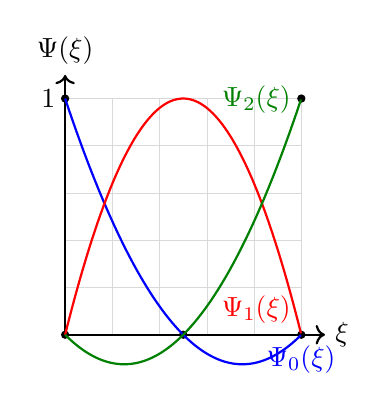
\begin{tikzpicture}[scale=3]
		% Grid
		\draw[very thin,color=gray!30] (0,0) grid[step=0.2] (1,1);
		\draw[->,thick] (0,0) -- (1.1,0) node[right] {\(\xi\)};
		\draw[->,thick] (0,0) -- (0,1.1) node[above] {\(\Psi(\xi)\)};

		% Reference points
		\fill (0,1) circle (0.5pt) node[left] {1};
		\fill (0.5,0) circle (0.5pt);
		\fill (1,0) circle (0.5pt);
		\fill (0,0) circle (0.5pt);
		\fill (1,1) circle (0.5pt);

		% Shape functions
		\draw[thick,blue,domain=0:1,samples=100] plot (\x,{2*\x*\x - 3*\x + 1})
		node[below] {\(\Psi_0(\xi)\)};
		\draw[thick,red,domain=0:1,samples=100] plot (\x,{-4*\x*\x + 4*\x})
		node[above left] {\(\Psi_1(\xi)\)};
		\draw[thick,green!50!black,domain=0:1,samples=100] plot (\x,{2*\x*\x - \x})
		node[left] {\(\Psi_2(\xi)\)};
	\end{tikzpicture}
	\caption{Quadratic Lagrange shape functions on the reference interval \([0,1]\).}
	\label{fig:quadratic-shape-functions}
\end{figure}

To get basis functions on a physical element \(K_k = [x_{2k}, x_{2k+2}]\), we use an \emph{affine mapping} \(\Phi_{K_k}: \hat K \to K_k\).
One convenient mapping is linear:
\[
	\Phi_{K_k}(\xi) = x_{2k} + \xi\, (x_{2k+2}-x_{2k}) \implies
	\begin{cases}
		\Phi_{K_k}(\xi=0) = x_{2k},     \\
		\Phi_{K_k}(\xi=0.5) = x_{2k+1}, \\
		\Phi_{K_k}(\xi=1) = x_{2k+2}.
	\end{cases}
\]
which sends \(\xi=\{0,0.5,1\}\) to \(\{x_{2k}, x_{2k+1}, x_{2k+2}\}\) respectively.

The local shape functions \(\phi_{k,\alpha}(x)\) on \(K_k\) are then defined by:
\[
	\phi_{k,\alpha}(x) = \Psi_\alpha(\xi), \quad \xi = \Phi_{K_k}^{-1}(x) = \frac{x-x_{2k}}{h_k}
\]
\[
	\phi_{k,\alpha}(x) = \Psi_\alpha\left(\frac{x-x_{2k}}{h_k}\right), \quad h_k = x_{2k+2}-x_{2k}.
\]
Because of the linear map, these \(\phi_{k,\alpha}(x)\) are still in \(\mathbb{P}_2\), just stretched or compressed to the element size.
Each local \(\phi_{k,\alpha}\) is supported only on element \(K_k\) and satisfies \(\phi_{k,\alpha}(x_{2k+\alpha})=1\) and \(\phi_{k,\alpha}(x) =0\) at the other two nodes of \(K_k\).

\subsection*{Global basis assembly}
The global basis functions \(\{\varphi_j(x)\}_{j=0}^{2M}\) are constructed from the local shapes by identifying them at shared nodes.
In practice, we label each global basis \(\varphi_j\) to correspond to node \(x_j\).
For example, \(\varphi_2(x)\) is the basis associated with the node \(x_2\), which is an endpoint of element \(K_1\) and \(K_0\);
\(\varphi_2\) is composed of the piece of \(\phi_{0,2}\) on \(K_0\) (which equals 1 at \(x_2\)) and the piece of \(\phi_{1,0}\) on \(K_1\), ensuring \(\varphi_2\) is continuous and piecewise quadratic.
Each interior node corresponds to a unique global basis function that may span one or two adjacent elements.

By construction, \(\varphi_i(x_j) = \delta_{ij}\), and any \(v_h \in V_h\) can be expanded as:
\[
	v_h(x) = \sum_{j \in \mathcal{N}_{int}} v_j\, \varphi_j(x),
\]
where the sum runs over all interior (free) nodes.

The boundary nodes \(x_0\) and \(x_{2M}\) are excluded in \(V_h\) because those basis functions would lie outside \(H^1_0\) (they would equal 1 at the boundary).
Thus we have \(2M-1\) basis functions for \(V_h\).

\subsection*{Assembly of Stiffness Matrix and Load Vector}
Using the Galerkin condition, we derive a linear system for the coefficients of \(u_h\).
Let \(\{ \varphi_j \}_{j=1}^{2M-1} \) be the global basis for \(V_h\).

We seek:
\[
	u_h(x) = \sum_{j=1}^{2M-1} u_j\, \varphi_j(x)
\]
that satisfies \(a(u_h,v) = F(v)\) for all \(v \in V_h\).
Plugging in \(v = \varphi_i\) and using linearity:

\begin{align*}
	a(u_h,\varphi_i) = \sum_{j} u_j\, a(\varphi_j,\varphi_i) = F(\varphi_i), \quad i=1,\dots,2M-1.
\end{align*}

This yields a linear system \(AU = F\) in matrix form, where the \emph{stiffness matrix} \(A\) and \emph{load vector} \(F\) are given by:
\begin{align*}
	A_{ij}  = a(\varphi_j,\varphi_i) & = \int_0^1 \varphi_j'(x)\,\varphi_i'(x)\,dx \\
	F_i     = F(\varphi_i)           & = \int_0^1 f(x)\,\varphi_i(x)\,dx
\end{align*}

\(A\) is symmetric and sparse: each basis \(\varphi_j\) has small support (at most two elements), so \(A_{ij}\neq 0\) only if \(\varphi_i, \varphi_j\) overlap on some element. 
In fact, each element contributes a \(3\times 3\) submatrix to \(A\).

We construct \(A\) by \emph{element-wise assembly}: sum up contributions from each element's local stiffness matrix.

\subsection*{Local element computations}
Consider one element \(K_k = [x_{2k}, x_{2k+2}]\) with length \(h_k = x_{2k+2}-x_{2k}\).
Let local basis \(\{\phi_{k,0},\phi_{k,1},\phi_{k,2}\}\) correspond to nodes \(\{x_{2k}, x_{2k+1}, x_{2k+2}\}\).
We compute the element stiffness matrix.
\[
A^{(k)}_{\alpha\beta} = \int_{K_k} \phi'_{k,\alpha}(x)\,\phi'_{k,\beta}(x)\,dx, \quad \alpha,\beta=0,1,2
\]
Using the reference element mapping simplifies this integration.
Under \(x = \Phi_{K_k}(\xi)\), we have \(dx = h_k\,d\xi\) and \(\frac{d\phi_{k,\alpha}}{dx} = \frac{1}{h_k}\frac{d\Psi_\alpha}{d\xi}\).
Thus:
\[
A^{(k)}_{\alpha\beta} 
= \int_{0}^{1} \frac{1}{h_k}\Psi'_{\alpha}(\xi)\,\frac{1}{h_k}\Psi'_{\beta}(\xi) \,h_k\,d\xi 
= \frac{1}{h_k^2}\int_{0}^{1} \Psi'_{\alpha}(\xi)\Psi'_{\beta}(\xi)\,d\xi.
\]

The reference integral \(\int_0^1 \Psi'_{\alpha}(\xi)\Psi'_{\beta}(\xi)d\xi\) is a constant (one can compute these values once, or use numerical quadrature).

Similarly, the local load vector entries are \(b^{(k)}_{\alpha} = \int_{K_k} f(x)\,\phi_{k,\alpha}(x)\,dx\).
Substituting \(x = x_{2k}+h_k\xi\):
\[b^{(k)}_{\alpha} = \int_{0}^{1} f(x_{2k}+h_k\xi)\,\Psi_{\alpha}(\xi)\,h_k\,d\xi.\]
This integral generally does not have a closed-form expression if \(f(x)\) is arbitrary, so we approximate it by numerical quadrature.

\subsubsection*{Numerical integration (quadrature)}
The assignment suggests \emph{Simpson's rule} as a convenient choice.
Simpson's rule on \([0,1]\) uses the points \(\{0, 0.5, 1\}\) (which happen to be the reference nodes) and weights \((1/6,\,4/6,\,1/6)\), and is exact for polynomials up to cubic degree. 
It turns out that Simpson's rule will integrate the quadratic basis functions times \(f\) with good accuracy (exact if \(f\) is up to degree 2, and generally very small error for smooth \(f\)). 

A nice benefit is that because \(\Psi_\alpha(\xi)\) is \emph{Lagrange basis}, \(\Psi_{\alpha}(\xi_\beta) = \delta_{\alpha\beta}\), the quadrature simplifies:

\begin{itemize}
	\item For the endpoint basis \(\Psi_0\), Simpson's rule gives:
	\[
	b^{(k)}_0 \approx \frac{h_k}{6}[f(x_{2k}) + 4f(x_{2k+1}) + f(x_{2k+2})] \Psi_0(0) = \frac{h_k}{6}[f(x_{2k})
	\] 
	(since \(\Psi_0(0)=1\), others zero at \(\xi=0,0.5,1\)).
	\item Likewise with midpoint:
	\[
	b^{(k)}_1 \approx \frac{4h_k}{6} f(x_{2k+1})
	\]
	\item and endpoint:
	\[
	b^{(k)}_2 \approx \frac{h_k}{6} f(x_{2k+2}) 	
	\]
\end{itemize}

In fact, Simpson's rule \emph{exactly} integrates \(f(x)\Psi_\alpha(\xi)\) if \(f\) is at most quadratic on the element, and provides a good approximation in general.
For the stiffness integrals, \(\phi'_{k,\alpha}\phi'_{k,\beta}\) is a polynomial of degree at most 2, so Simpson's rule actually integrates it exactly.
Thus, using Simpson's rule for all element integrals yields accurate results.
Alternatively, one could use 2-point Gaussian quadrature (exact for degree 3 integrands) or even analytic integration if desired.

\subsection*{Assembly procedure}
We accumulate each element's contributions into the global matrix \(A\) and vector \(b\). A high-level outline of the assembly algorithm is:
\begin{itemize}
	\item \emph{Mesh data structures:} 
	prepare an array of node coordinates \mintinline{python}{x_nodes[0...2M]}, and a connectivity list for elements (for each element \(k\), store the global node indices of its three nodes, e.g. \mintinline{python}{[2k, 2k+1, 2k+2]}).
	\item Initialize global matrix of size \(A \in \mathbb{R}^{(2M+1)\times(2M+1)}\) and global load vector of length \(\mathbf{b} \in \mathbb{R}^{2M+1}\) to zero. 
	(We include all nodes initially, including boundaries.)
	\item Loop over each element \(K_k\):
	      \begin{enumerate}
		      \item Compute \(h_k = x_{2k+2} - x_{2k}\).
		      \item  Compute the \(3 \times 3\) \textbf{local stiffness matrix} \mintinline{python}{A_loc} with entries
		            \[A^{(k)}_{\alpha\beta} = \frac{1}{h_k}\int_0^1 \Psi'_{\alpha}(\xi)\Psi'_{\beta}(\xi)d\xi.\]
		            (These reference integrals can be precomputed once; for quadratic basis, the result is often given in textbooks.)
		      \item Compute the \textbf{local load vector} \mintinline{python}{b_loc} of length 3, e.g. by Simpson's rule:
			  		\begin{align*}			  			
		            b^{(k)}_0 &= \frac{h_k}{6}[f(x_{2k}) + 4f(x_{2k+1}) + f(x_{2k+2})],\\
		            b^{(k)}_1 &= \frac{h_k}{6}[f(x_{2k}) + 4f(x_{2k+1}) + f(x_{2k+2})] \quad\text{(with appropriate weights, see above)},\\
		            b^{(k)}_2 &= \frac{h_k}{6}[f(x_{2k}) + 4f(x_{2k+1}) + f(x_{2k+2})].
					\end{align*}
		            (Note: Actually, the correct Simpson formula is \(h_k/6 [f(x_{2k}) + 4f(x_{2k+1}) + f(x_{2k+2})]\), and then multiplied by the shape function value at those points.
		            Because \(\phi_{k,0}(x_{2k})=1\) and zero at other nodes, the \(\phi_{k,0}\) integral reduces to \(h_k/6 f(x_{2k})\), etc.
		            For clarity one can just evaluate \(f\) at each node and multiply by the appropriate weight for each local basis.)
		      \item \textbf{Add to global matrix:} for each local index \(\alpha,\beta\), let \mintinline{python}{I = global_node_index[k][alpha]} and \mintinline{python}{J = global_node_index[k][beta]}.
		            Add \(A^{(k)}_{\alpha\beta}\) to \(A[I,J]\).
		            Similarly, add \(b^{(k)}_{\alpha}\) to \(b[I]\).
	      \end{enumerate}
	\item  After the loop, \mintinline{python}{A} and \mintinline{python}{B} hold the \emph{assembled} system incorporating all elements.
\end{itemize}

At this stage, the system still includes the boundary nodes. We have \(A\) of size \((2M+1)\times(2M+1)\) and \(b\) of length \(2M+1\), but we know \(u_h(0)=u_h(1)=0\) a priori. 
The easiest way to enforce the Dirichlet boundary conditions \(u_h(0)=u_h(1)=0\) is to \textbf{eliminate those degrees of freedom}. 
We can do this by removing the first and last rows and columns of \(A\), and the first and last entry of \(b\).
This leaves us with a reduced linear system of size \((2M-1)\times(2M-1)\) for the unknown coefficients \(U_1,\dots,U_{2M-1}\) corresponding to interior nodes. (By removing rows/cols, we are essentially applying the conditions \(U_0=U_{2M}=0\) and ensuring the equations associated with those nodes are dropped, which is valid since those basis functions are not in \(V_h\).)

\subsection*{Matrix properties}
The resulting stiffness matrix \(A\) is symmetric positive-definite (SPD). 
The linear system \(A U = b\) can thus be solved with e.g. the conjugate gradient method or a direct Cholesky factorization. 
Because this is a 1D second-order problem, \(A\) will also be banded (bandwidth 3 in this case, since each interior node connects to at most its two neighbors). 
For efficiency, it's good to use a sparse matrix representation.

\subsection*{Implementation in Python}
When coding the FEM solver, it's important to write modular functions and re-use them for both problems. 
Key components include mesh generation, basis function definitions, element integration, assembly, and linear solver. 
Here are some guidelines for implementing the Poisson solver:
\begin{itemize}
	\item \textbf{Mesh representation:}
	      Represent the list of node coordinates (including boundaries and midpoints). You can generate a uniform mesh easily by dividing \([0,1]\) into \(M\) equal subintervals and inserting midpoints.
	      For a non-uniform mesh, you might specify the positions of the even-indexed nodes (element boundaries) and then compute midpoints.
	      For example, if \mintinline{python}{x_even = [0, x2, x4, ..., 1]} is a list of element boundaries, then the full node list is \mintinline{python}{x_nodes = [0, (x2)/2, x2, (x2+x4)/2, x4, ... 1]}.
	      Ensure the nodes are in sorted order. You can store connectivity as a list of elements, where each element is a tuple of three global node indices.
	\item \textbf{Reference shape functions:}
	      It's convenient to have functions for the reference shape values and derivatives.
	      For example, implement \(\Psi_0(\xi), \Psi_1(\xi), \Psi_2(\xi)\) and their derivatives. (In code, you could hard-code these small polynomials or use a symbolic approach, but hard-coding is fine here.)
	      These can be used to compute local matrix entries via quadrature.
	\item \textbf{Local matrix assembly:}
	      Compute local stiffness and load.
	      You can either derive explicit formulas for the local stiffness matrix entries (for quadratic elements in 1D, these are known constants times \(1/h\)) or simply perform the quadrature.
	      For instance, using Simpson's rule: sample the derivative of shapes at \(\xi=0,0.5,1\) for stiffness, and sample \(f(x)\) at element nodes for the load. Pseudo-code:
\end{itemize}

\begin{algorithm}[H]
	\caption{Local Element Matrix Assembly for P2 FEM}
	\DontPrintSemicolon
	\KwIn{Element index \(k\), node coordinates \(x_{nodes}\), source function \(f(x)\)}
	\KwOut{Local stiffness matrix \(A_{loc}\), local load vector \(b_{loc}\)}

	\(h \leftarrow x_{nodes}[2k+2] - x_{nodes}[2k]\) \tcp*{Element length}

	\tcp{Initialize local matrices}
	\(A_{loc} \leftarrow \text{zeros}(3,3)\) \;
	\(b_{loc} \leftarrow \text{zeros}(3)\) \;

	\tcp{Precompute shape function derivatives at quadrature points}
	{
		$dPsi \leftarrow \begin{bmatrix}
				-3 & -1 & 1  \\
				4  & 0  & -4 \\
				-1 & 1  & 3
			\end{bmatrix}$
		\tcp*{Values at $\xi=0,0.5,1$}
	}

	\(w \leftarrow [1/6, 4/6, 1/6]\) \tcp*{Simpson weights}

	\tcp{Assemble stiffness matrix}
	\For{\(\alpha \leftarrow 0\) \KwTo \(2\)}{
		\For{\(\beta \leftarrow 0\) \KwTo \(2\)}{
			\(ref\_int \leftarrow \sum_{q=0}^2 w[q] \cdot dPsi[\alpha,q] \cdot dPsi[\beta,q]\) \;
			\(A_{loc}[\alpha,\beta] \leftarrow \frac{1}{h} \cdot ref\_int\)
		}
	}

	\tcp{Compute load vector}
	\(f_{vals} \leftarrow [f(x_{nodes}[2k]), f(x_{nodes}[2k+1]), f(x_{nodes}[2k+2])]\) \;
	\For{\(\alpha \leftarrow 0\) \KwTo \(2\)}{
		\(b_{loc}[\alpha] \leftarrow \frac{h}{6} \cdot f_{vals}[\alpha]\) \tcp*{Using Lagrange property}
	}

	\Return{\(A_{loc}, b_{loc}\)}
\end{algorithm}

\begin{minted}[linenos,frame=lines]{python}

\end{minted}

\paragraph{Global assembly}
Initialize a sparse matrix data structure (e.g. use SciPy's \mintinline{python}{lil_matrix} or similar) for \(A\) of size \((2M+1)\times(2M+1)\) and a NumPy array for \(b\).
Loop through each element and add the contributions: for local index \(\alpha\) with corresponding global index \mintinline{python}{I = element_nodes[k][alpha]}, add \(b^{(k)}_\alpha\) to \mintinline{python}{b[I]}.
For each pair \((\alpha,\beta)\), add \(A^{(k)}_{\alpha\beta}\) to \mintinline{python}{A[I,J]} with \mintinline{python}{J = element_nodes[k][\beta]}.
\begin{minted}[linenos,frame=lines]{python}
def assemble_poisson(M, x_nodes, f):
	"""Assemble global stiffness matrix and load vector for Poisson problem."""
	
	# Initialize global matrix and vector
	A = lil_matrix((2*M+1, 2*M+1))  # Sparse matrix
	b = np.zeros(2*M+1)              # Load vector
	
	# Loop over each element
	for k in range(M):
		A_loc, b_loc = assemble_element_matrices(k, x_nodes, f)
		
		# Add local contributions to global matrix and vector
		for alpha in range(3):
			I = element_nodes[k][alpha]
			b[I] += b_loc[alpha]
			for beta in range(3):
				J = element_nodes[k][beta]
				A[I,J] += A_loc[alpha,beta]
	
	return A, b
\end{minted}


\paragraph{Apply boundary conditions}
Remove or zero-out the Dirichlet degrees of freedom.
Since \(u(0)=u(1)=0\), you can remove the first and last rows and columns of \(A\) and the first and last entry of \(b\).
If using SciPy, you might do this by slicing:
\begin{minted}[linenos,frame=lines]{python}
A_reduced = A[1:-1, 1:-1]  # Remove first and last rows/columns
b_reduced = b[1:-1]        # Remove first and last entries
\end{minted}
Alternatively, set the rows corresponding to \(x_0,x_{2M}\) to identity and adjust \(b\) to 0 at those positions (the removal approach is simpler in this zero-Dirichlet case).
\begin{minted}[linenos,frame=lines]{python}
A[0, :] = 0
A[0, 0] = 1
A[-1, :] = 0
A[-1, -1] = 1
b[0] = 0
b[-1] = 0
\end{minted}

\paragraph{Solve linear system}
Use a sparse linear solver. 

For example, \mintinline{python}{scipy.sparse.linalg.spsolve(A_reduced, b_reduced)} will solve the system efficiently.
This yields the coefficient vector \(U\) for interior nodes.
You can then insert the known boundary values (0) to reconstruct the full solution vector of length \(2M+1\) if needed for evaluation.
\begin{minted}[linenos,frame=lines]{python}
from scipy.sparse.linalg import spsolve
# Solve the linear system
U_reduced = spsolve(A_reduced, b_reduced)
# Reconstruct full solution vector
U_full = np.zeros(2*M+1)
U_full[1:-1] = U_reduced
# U_full now contains the solution at all nodes, including boundaries
U_full[0] = 0
U_full[-1] = 0
\end{minted}

\paragraph{Modularity}
Keep the assembly and solver general. For instance, write a function \mintinline{python}{assemble_poisson(M, node_coords, f_function)} that returns the matrix and vector, and a function \mintinline{python}{solve_poisson(A, b)} that applies boundary conditions and solves.
This modular design pays off, because for the optimal control problem, you will reuse the assembly of the stiffness matrix (and also assemble a mass matrix similarly).

\subsection{Error Analysis and Convergence}
For the Poisson problem, since we are using a polynomial degree \(p=2\) (quadratic) basis, we expect a certain rate of convergence as the mesh is refined.
The exact theory (from finite element error analysis) states that if the true solution \(u\) is sufficiently smooth (here \(u\in H^1_0\cap H^3\) typically), the \(H^1\)-norm error should behave like \(O(h^p) = O(h^2)\) and the \(L^2\)-norm error like \(O(h^{p+1}) = O(h^3)\) for quasi-uniform mesh.
Using known results (e.g. from the course notes by Curry, Lemmata 4.3 and 4.4), one can show \(\|u - u_h\|_{L^2} \le C\,h^3 \|u\|_{H^3}\) (for some constant \(C\) depending on the solution's third derivative) if the mesh size \(h\) is the maximum element length. Thus we anticipate third-order convergence in the \(L^2\) norm. The \(H^1\) norm error \(\|u-u_h\|_{H^1}\) is expected to be \(O(h^2)\).

\paragraph{Verifying numerically}
To confirm this, one can perform a convergence test.
Choose a test problem with known exact solution \(u(x)\). For example, take \(f(x)=1\) on \((0,1)\) with \(u(0)=u(1)=0\). The exact solution is \(u(x) = \frac{x(1-x)}{2}\) (since \(-u''=1\) integrates to a parabola) – this \(u(x)\) is a smooth function in \(H^3\). Run the solver on a sequence of meshes (e.g. \(M=4,8,16,32\) elements) and compute the \(L^2\) error \(\|u - u_h\|_{L^2}\) and \(H^1\) error \(\|u-u_h\|_{H^1}\). The \(L^2\) norm can be approximated by numerical integration: \(\|u - u_h\|_{L^2} \approx \sqrt{\sum_{k=0}^{M-1}\int_{K_k} (u(x)-u_h(x))^2 dx}\) (again Simpson's rule or a finer quadrature can be used per element for this calculation). Then check the rate: if you halve \(h\) (double number of elements), the \(L^2\) error should roughly scale by about \(1/8\) (since \(h^3\) is eight times smaller when \(h\) halves). Similarly, the \(H^1\) error should scale by about \(1/4\) (\(h^2\) behavior). In a log-log plot of error vs. \(h\), \(L^2\) error should have slope ~3, \(H^1\) error slope ~2. Documenting this convergence behavior validates that the implementation is correct and that the theoretical order is achieved.

When writing the report, you might not need to include all the code or trivial verification plots, but you should\textbf{mention that you tested the implementation} on known solutions to ensure correctness (as advised).
You can then confidently proceed to more interesting cases for the report's results, knowing your code is working and converging correctly.

\section{Finite Element Discretization of the OCP}
Using the quadratic Lagrange space \(V_h = X_h^2 \cap H^1_0(0,1)\) (dimension \(n=2N-1\) for \(N\) elements), we express the state \(y_h(x)\) and control \(u_h(x)\) in the FEM basis.
Let \(\{\phi_i\}_{i=1}^n\) be the interior basis functions. The discrete objective functional \(G(y,u)\) follows from the continuous \(J(y,u)\).

\subsection{Discrete functional}

\[
	G(y,u) \;=\; \frac{1}{2}\,(y - \bar y_d)^T M\, (y - \bar y_d)\;+\;\frac{\alpha}{2}\,u^T M\,u,
\]

where \(y, u \in \mathbb{R}^n\) are the coefficient vectors of \(y_h, u_h\) in the \(V_h\) basis, and \(\bar y_d\) is the interpolated target vector.

Here \(M\) is the mass matrix with entries \(M_{ij}=\int_0^1 \phi_i(x)\phi_j(x)\,dx\). The first term \(\frac{1}{2}\|y_h - \bar y_d\|_{L^2}^2\) is \((y-\bar y_d)^T M (y-\bar y_d)/2\), and the second term \(\frac{\alpha}{2}\|u_h\|_{L^2}^2\) is \(\alpha\,u^T M u/2\).

\subsection{Discrete constraint}

The FE weak form requires \(a(y_h,v) = \langle u_h,v\rangle\) for all \(v\in V_h\), where \(a(y,v)=\int_0^1 y'(x)v'(x)\,dx\). In matrix form this gives the linear constraint

\[
	B\,y \;=\; F\,u,
\]

with\textbf{\(B\) the stiffness matrix} \(K\) (entries \(K_{ij}=\int_0^1 \phi_i'(x)\phi_j'(x)\,dx\)) and\textbf{\(F\) the mass matrix} \(M\).  In other words, \(By=Fu\) is the algebraic system \(K\,y = M\,u\), which corresponds to the discrete PDE \(-y_h''=u_h\) with \(y_h(0)=y_h(1)=0\). (This follows since \(K y\) represents the left-hand side \(\int y'_h v'_h\) in the basis, and \(M u\) the right-hand side \(\int u_h v_h\).)

\paragraph{Answer for 1}
\(G(y,u)=\frac12 (y-\bar y_d)^T M (y-\bar y_d) + \frac{\alpha}{2} u^T M u\), with \(B=K\) (stiffness matrix) and \(F=M\) (mass matrix), so the constraint is \(K y = M u\).

\subsection{KKT Optimality System via Lagrange Multipliers}

We introduce a Lagrange multiplier vector \(\lambda\in\mathbb{R}^n\) (representing the discrete\textbf{adjoint state}). The Lagrangian of the constrained problem is:

\[
	\mathcal{L}(u,y,\lambda) \;=\; G(y,u)\;-\;\lambda^T(B y - F u)\,,
\]

which in full is: \(\; \mathcal{L}(u,y,\lambda) = \frac{1}{2}(y-\bar y_d)^T M (y-\bar y_d) + \frac{\alpha}{2} u^T M u \;-\;\lambda^T(Ky - M u)\,. \)

Setting the partial derivatives to zero (first-order optimality conditions gives the Karush–Kuhn–Tucker system:

\begin{itemize}
	\item \textbf{State equation (from \(\nabla_\lambda \mathcal{L}=0\)):}
	      \[By - Fu = 0 \quad\Longrightarrow\quad K\,y - M\,u = 0.\]
	      This recovers the discrete state equation \(K y = M u\) (the constraint).
	\item \textbf{Adjoint equation (from \(\nabla_y \mathcal{L}=0\)):}
	      \[\partial \mathcal{L}/\partial y = M(y - \bar y_d) - K^T \lambda = 0.\]
	      Since \(K\) is symmetric positive-definite, \(K^T=K\). Thus,
	      \[M(y - \bar y_d) \;=\; K\,\lambda.\]
	      This is the\textbf{adjoint} equation relating \(\lambda\) and the state error \(y-\bar y_d\).

	\item \textbf{Optimality condition for \(u\) (from \(\nabla_u \mathcal{L}=0\)):}
	      \[\partial \mathcal{L}/\partial u = \alpha\, M u - F^T \lambda = 0.\]
	      Here \(F^T=M^T=M\) (mass matrix is symmetric), so
	      \[\alpha\, M u \;-\; M\,\lambda = 0 \;\;\Longrightarrow\;\; \alpha\,M\,u = M\,\lambda.\]
	      Because \(M\) is invertible on the interior DOFs, this implies \(\lambda = \alpha\,u\).  (Equivalently, \(\alpha u_h(x) + \lambda_h(x) = 0\) in function form, meaning the optimal control is \(u_h=-\frac{1}{\alpha}\lambda_h\).)
\end{itemize}

We now have three equations:
\[
	K y - M u = 0, \qquad M(y - \bar y_d) = K\lambda, \qquad \lambda = \alpha\,u.
\]

We can eliminate \(\lambda\) and either \(y\) or \(u\) to solve for the optimal \((y,u)\). Substituting \(\lambda=\alpha u\) into the adjoint eq.:
\[M(y - \bar y_d) = K(\alpha u) = \alpha\,K\,u.\]
Also, the state eq. gives \(K y = M u\). Using these two, we can derive a coupled linear system in \(y\) and \(u\). One convenient form is to keep both \(y\) and \(u\) as unknowns. Combining the equations, we get the\textbf{saddle-point system}:

\[
	\begin{pmatrix} K & -\,M      \\[6pt]
                M & \alpha\,K\end{pmatrix}
	\begin{pmatrix}
		y \\[3pt] u
	\end{pmatrix} =
	\begin{pmatrix}
		0 \\[3pt]
		M\,\bar y_d
	\end{pmatrix}.
\]

This \(2n\times 2n\) linear system is obtained by writing \(K y - M u = 0\) as the first block row, and \(M y - \alpha K u = M \bar y_d\) (which is the adjoint equation \(M y - M \bar y_d + \alpha K u=0\) rearranged) as the second block row.  Solving this system yields the optimal coefficients \(y^\star\) and \(u^\star\).  (Alternatively, one can eliminate one variable: for example, from \(K y=M u\) we get \(u = K^{-1} M y\), and substituting into the adjoint equation gives \((M + \alpha\,K) y = M\,\bar y_d\). This reduced \(n\times n\) system can be solved for \(y\), then \(u\) recovered.)

\paragraph{Answer for 2:}
The Lagrangian is \(\;L(u,y,\lambda) = \frac{1}{2}(y-\bar y_d)^T M (y-\bar y_d) + \frac{\alpha}{2} u^T M u - \lambda^T(Ky - M u)\;\).
Setting gradients zero:
\begin{enumerate}
	\item \(\nabla_y L: M(y-\bar y_d) - K^T\lambda = 0\),
	\item \(\nabla_u L: \alpha\,M u - M^T\lambda = 0\),
	\item \(\nabla_\lambda L: K y - M u = 0\).
\end{enumerate}


Using \(K^T=K\) and \(M^T=M\), the KKT system is:
\[ K y = M u, \qquad M(y-\bar y_d) = K\lambda, \qquad \alpha\,M u = M\lambda. \]
Eliminating \(\lambda\) gives \(M(y-\bar y_d) + \alpha K u = 0\) and \(K y - M u = 0\). The final linear system for \((y,u)\) is:
\[ \begin{pmatrix}K & -M\\ M & \alpha K\end{pmatrix}\begin{pmatrix}y\\ u\end{pmatrix} = \begin{pmatrix}0\\ M\,\bar y_d\end{pmatrix}, \]
which can be solved for the optimal state \(y_h\) and control \(u_h\).

\subsection{Python Implementation of the FEM Solver}
To solve the optimal control system, we assemble the finite element matrices and then solve the above linear system. The steps are:

\subsubsection{Mesh and basis}
Partition \([0,1]\) into \(N\) elements. Using quadratic Lagrange basis functions, assemble the\textbf{stiffness matrix} \(K\in\mathbb{R}^{n\times n}\) and\textbf{mass matrix} \(M\in\mathbb{R}^{n\times n}\) for the interior DOFs. In code, this involves computing element matrices (via Gaussian quadrature or exact formulas) and summing into global matrices.

\subsubsection{Interpolate \(y_d\)}
Compute the vector \(\bar y_d\in\mathbb{R}^n\) by interpolating the target \(y_d(x)\) at the interior nodes (and mid-nodes) of the mesh. This ensures \(\bar y_d \in V_h\).

\subsubsection{Form linear system}
Construct the saddle-point matrix and RHS as derived above. For example, using block-matrix notation, one can form \(A = \begin{pmatrix}K & -M;~M & \alpha K\end{pmatrix}\) and \(b = \begin{pmatrix}0 \\ M\,\bar y_d\end{pmatrix}\). In implementation, \(A\) can be assembled blockwise or solved by eliminating one of the variables.

\subsubsection{Solve for \((y,u)\)}
Solve the linear system for the coefficient vectors \(y\) and \(u\). This can be done with a direct solver (since \(A\) is symmetric indefinite but well-conditioned for \(\alpha>0\)) or by solving the reduced system \((M + \alpha K)y = M\bar y_d\) for \(y\) then recovering \(u = M^{-1}K y\).

Below is a pseudo-code snippet illustrating the solver:
\begin{minted}[linenos,frame=lines]{python}
# Assume K, M are assembled numpy arrays of shape (n,n), and y_d_vec is the interpolated target (length n).
import numpy as np
n = K.shape[0]
# Form the KKT matrix A and right-hand side vector rhs
A = np.block([[K, -M],
              [M,  alpha*K]])
rhs = np.concatenate([np.zeros(n), M.dot(y_d_vec)])
# Solve for [y; u] (length 2n vector)
sol = np.linalg.solve(A, rhs)
y_coeff = sol[:n]   # optimal y_h coefficients
u_coeff = sol[n:]   # optimal u_h coefficients
\end{minted}

This yields the discrete optimal state \(y_h(x)\) and control \(u_h(x)\) in the finite element basis. One can then evaluate or plot these solutions as piecewise quadratics on the mesh.\footnote{In our implementation, we reused the FEM assembly from Problem 1 to build \(M\) and \(K\), then solved the system for each scenario.}

\subsection{Numerical Results for Different Target Profiles}
We tested the solver for three target functions:

\begin{enumerate}
	\item \textbf{\(y_d(x)=\frac{1}{2}x(1-x)\) (Parabolic target in \(H^1_0\)):} This target is smooth and satisfies the boundary conditions (\(y_d(0)=y_d(1)=0\)), so it is \textbf{feasible} as an \(H^1_0\) function. For typical moderate \(\alpha\) (e.g., \(10^{-3}\)), the optimal solution \(y_h\) is very close to \(y_d\) throughout \([0,1]\), and the control \(u_h\) is close to the “exact” forcing \(-y_d''(x)=1\). As \(\alpha\) becomes large (costly control), the optimizer scales back the control. For example, with \(\alpha=1\), we found \(u_h(x)\approx 0.5\) (a roughly constant control half as strong as the ideal) and accordingly \(y_h(x)\approx 0.5\,y_d(x)\) (about half the target profile). This makes sense: when control is expensive, the solution compromises by not reaching the full target amplitude. On the other hand, as \(\alpha\to 0\) (cheap control), \(u_h\) increases toward the exact needed forcing. In fact, for \(\alpha\) very small (\(10^{-6}\) or \(10^{-8}\)), we obtained \(y_h(x)\approx y_d(x)\) to within plotting accuracy, and \(u_h(x)\approx 1\) across the domain. In summary, for this \textit{\(H^1_0\)-compatible} target, the optimal state converges to the target and the control remains well-behaved (approaching the smooth function \(1\)) as \(\alpha\to 0\).

	\item \textbf{\(y_d(x)=1\) (Constant target, not in \(H^1_0\)):} This target does \textbf{not} satisfy the boundary condition (\(y_d(0)=y_d(1)=1\neq 0\)), so it is \textit{not attainable} by any \(H^1_0\) function. The optimal solution reflects this. For large \(\alpha\) (e.g., \(\alpha=0.1\) or \(1\)), the algorithm chooses to apply very little control. In fact, as \(\alpha\) increases, the optimal \(u_h\) tends to \(0\), and \(y_h\) tends to the zero state (which incurs a large \(L^2\) error, but saves control cost). For example, with \(\alpha=1\), we found \(u_h\) was nearly zero and \(y_h\) remained very low (peaking around \(0.1\) in the interior). For small \(\alpha\) (cheap control), the optimizer tries to force \(y_h\) to match 1 on \((0,1)\) as closely as possible. However, \(y_h(0)\) and \(y_h(1)\) must remain 0, so what happens is that \textbf{very large control values} concentrate near the boundaries \(x=0\) and \(x=1\) to create steep boundary layers. For \(\alpha=10^{-6}\), our solution had \(u_h\) on the order of \(10^5\) near \(x=0\) and \(x=1\) (within the first and last few mesh cells), with \(u_h\) smaller in the interior. This strong forcing raised the interior of \(y_h\) close to 1. Indeed, \(y_h(x)\approx 1\) for most of \(0<x<1\), but it drops sharply to \(0\) at the boundaries. The transition occurs in a thin region near the edges, where \(y_h\) has a large gradient. These trends intensify as \(\alpha\to 0\): \(u_h\) grows without bound at the boundaries, and \(y_h\) approaches 1 on \((0,1)\) (but will always satisfy \(y_h(0)=y_h(1)=0\)). This illustrates the case of an \textbf{inadmissible target} – the algorithm does its best, but cannot exactly achieve \(y_d\). The \(L^2\) error \(\|y_h-y_d\|_{L^2}\) decreases as \(\alpha\) decreases (since interior \(y_h\) gets closer to 1), but the cost is unbounded control peaks.

	\item \textbf{\(y_d(x)\) = characteristic of \([1/4,3/4]\) (Discontinuous target):} This target is \textbf{not continuous}, hence not in \(H^1_0\). Its interpolation \(\bar y_d\) in the finite element space will be a continuous approximation of a step (a steep S-shaped curve that goes from 0 to 1 over a small interval around \(x=0.25\), and from 1 back to 0 around \(x=0.75\)). We observe behavior similar to case (ii) at the points of discontinuity. For large \(\alpha\), the optimal solution again avoids expensive control – with \(\alpha=1\) we found \(u_h\approx 0\), and thus \(y_h\approx 0\) (since the best “do nothing” state given homogeneous BC is zero everywhere, which in this case matches the target over \([0,0.25]\cup[0.75,1]\) but is far from the target on \([0.25,0.75]\)). For smaller \(\alpha\), the control will try to reduce the error on the middle interval. With \(\alpha=10^{-3}\), for instance, \(y_h\) rises a bit in \((0.25,0.75)\) but remains significantly below 1. For very small \(\alpha\) (\(10^{-6}\) or \(10^{-8}\)), the optimal \(u_h\) develops \textbf{two concentrated spikes}: one positive near \(x\approx 0.25\) and one negative near \(x\approx 0.75\). These correspond to forcing the state \(y_h\) up and then back down. The effect on \(y_h\) is that it becomes approximately 0 on \([0,0.25]\), then rapidly increases to \(\approx 1\) by slightly inside the interval \((0.25,0.75)\), stays near 1 in the middle, and then drops sharply to 0 near \(x=0.75\). In other words, \(y_h\) approximates the discontinuous target with a \textbf{smoothed “hat” profile}: the transitions at 1/4 and 3/4 are smooth but extremely steep for small \(\alpha\). Again, because \(y_d\) is not in the admissible set, \(u_h\) grows without bound (the smaller the cost parameter, the steeper – and larger in magnitude – the spikes). The optimal state \(y_h\) converges to a limit shape (the best \(H^1_0\) approximation of the step function) as \(\alpha\to 0\), which has small boundary-layer regions around \(0.25\) and \(0.75\). The interior of \(y_h\) approaches the target (value 1 on \([0.25,0.75]\)), while the jumps are smoothed out over vanishingly small intervals.
\end{enumerate}

\subsection{Effect of the Cost Parameter \texorpdfstring{\(\alpha\)}{alpha}}

Our experiments confirm the typical behavior of PDE-constrained optimizations:

\paragraph{Large \(\alpha\) (e.g. \(10^{-2}\) to \(1\))}
The term \(\frac{\alpha}{2}\|u_h\|^2\) dominates, so the optimal control tends to be\textbf{small}. The solution prioritizes reducing control effort at the expense of a larger state error. In the extreme \(\alpha\to\infty\), we get \(u_h\to 0\) and thus \(y_h\to 0\) (since no forcing is applied, the state stays at the homogeneous solution). In cases (ii) and (iii) with large \(\alpha\), we indeed saw \(y_h\) remain near 0 (far from the desired profile) because any attempt to reach \(y_d\) was too expensive. In case (i) (where \(y_d\) itself is small in magnitude), \(y_h\) also scaled down significantly as \(\alpha\) increased. This behavior is sensible: when control is very costly, the optimizer accepts a large mismatch rather than spend effort to reduce it.
\paragraph{Small \(\alpha\) (e.g. \(10^{-6}\) to \(10^{-8}\))}
Now the state-fit term \(\frac{1}{2}\|y_h-\bar y_d\|^2\) dominates, so the optimizer uses\textbf{aggressive control} to drive \(y_h\) towards \(y_d\). If \(y_d\) is attainable (\(y_d\in H^1_0\)), the limit \(\alpha\to 0\) yields \(y_h \to y_d\) exactly and \(u_h \to\) the exact control needed (which remains bounded). This was the case for (i): as \(\alpha\) decreased, \(y_h\) nearly coincided with \(y_d\) and \(u_h\) approached the smooth function \(1 = -y_d''\). However, if \(y_d\) is not in \(H^1_0\) (cases (ii) and (iii)), then \(y_d\) cannot be achieved by any finite \(y_h\). The algorithm then tries to approximate \(y_d\) as closely as possible, which entails \(u_h\) growing without bound in the limit \(\alpha\to 0\). In practice, for very small \(\alpha\) we observed extremely large control values at the locations of infeasibility (boundary points for case (ii), and discontinuity points for case (iii)). The optimal \(y_h\) approaches the “closest” \(H^1_0\) function to \(y_d\). For case (ii), that limit function is a sequence of states that get closer and closer to 1 in the interior (but always 0 at the boundary). For case (iii), the limit is a continuous function that is 0 at \(x=0,1\), \(\approx 1\) on \([0.25,0.75]\), with very steep ramps at the edges of that interval. Thus, when \(y_d \notin H^1_0\), decreasing \(\alpha\) yields diminishing returns in state accuracy – the interior error goes to zero, but \(y_h\) will never exactly equal \(y_d\) and the control norm \(\|u_h\|_{L^2}\) blows up. In contrast, when \(y_d\in H^1_0\), small \(\alpha\) leads to excellent tracking of the target with a well-behaved control.

In summary, \(\alpha\) acts as a \textbf{regularization parameter} balancing fidelity to \(y_d\) vs. control effort.
Large \(\alpha\) forces \(u_h\) toward 0 (under-control), while small \(\alpha\) drives \(y_h\) toward \(y_d\) at the expense of large \(u_h\). The qualitative difference between cases (i) vs. (ii)/(iii) underscores the importance of the target's admissibility: if \(y_d\) violates the PDE constraints (boundary conditions or smoothness), the optimal control will attempt to “fix” that by becoming very large (a phenomenon akin to approximating a nonsmooth function with smoother functions, leading to Gibbs-like overshoots or boundary layers). The results we obtained align with the theoretical expectations for (c1) and (c2), confirming that for \(y_d\in H^1_0\), \(u_h\) remains bounded as \(\alpha\to 0\), whereas for \(y_d\notin H^1_0\), \(u_h\) grows and \(y_h\) converges to the \(H^1_0\)-projection of \(y_d\).
The plots of \(y_h\) and \(u_h\) for the different cases and \(\alpha\) values (discussed above) illustrate these trends clearly.

\section{Problem 2: Optimal Control Problem (Poisson Constraint)}

\subsection{Problem Statement and Variational Formulation}
In the second part, we tackle an\textbf{optimal control problem} where the state equation is the same Poisson equation as above.

We have a \emph{state} \(y(x)\) (e.g. temperature in a rod) governed by \(-y'' = u\) on \((0,1)\) with \(y(0)=y(1)=0\).
Here \(u(x)\) is the \emph{control} (a distributed heat source).
We are given a desired state profile \(y_d(x)\) and a positive parameter \(\alpha\) that penalizes the cost of control.
The goal is to find a control \(u\) that makes \(y\) as close as possible to \(y_d\) while keeping control effort moderate.
This is formulated as the minimization problem:
\[\min_{y,u} \; J(y,u) = \frac{1}{2}\int_0^1 (y(x) - y_d(x))^2\,dx + \frac{\alpha}{2}\int_0^1 u(x)^2\,dx,\]
subject to the constraint \(-y''(x) = u(x)\), \(y(0)=y(1)=0\).

The two terms in \(J\) represent: (1) the\textbf{tracking error} – a least-squares measure of how far \(y\) is from the desired state \(y_d\), and (2) the\textbf{control cost} – a Tikhonov regularization term penalizing large controls. The weight \(\alpha > 0\) governs the trade-off: a small \(\alpha\) means we prioritize matching \(y_d\) more (allowing stronger control), while a large \(\alpha\) makes control expensive, favoring a solution with smaller \(u\) even if \(y\) deviates from \(y_d\).

This problem is a PDE-constrained optimization. In theory, one can derive the optimality conditions by introducing an adjoint variable. The continuous optimality system would consist of the state equation, an adjoint equation \(-\lambda'' = y - y_d\) with \(\lambda(0)=\lambda(1)=0\) for the adjoint (Lagrange multiplier enforcing the state equation), and the optimality condition \(\lambda + \alpha\,u = 0\) (which links the adjoint to the control). We will derive the\textbf{discrete} analog of this using the finite element approach.

\subsection{Finite Element Discretization and Matrix Formulation}
We will approximate the optimal control problem using the same finite element space \(V_h\) as before for both the state \(y_h\) and (for simplicity) the control \(u_h\). In practice, \(u\) only needs to lie in \(L^2(\Omega)\), but taking \(u_h \in V_h\) (which is \(H^1_0\)) is a common choice that simplifies implementation (the control will also automatically satisfy zero at boundaries, which is not actually required physically, but in our discrete setup it is fine). So we seek \(y_h, u_h \in V_h\) that minimize
\[J_h(y_h, u_h) = \frac{1}{2}\|y_h - \bar{y}_d\|^2_{L^2} + \frac{\alpha}{2}\|u_h\|^2_{L^2},\]
subject to the discrete \emph{weak} constraint:

\[
	a(y_h, v) = {\langle u_h, v \rangle}_{L^2}\quad \forall v \in V_h
\]


Here \(\bar{y}_d\) is the projection or interpolation of \(y_d\) onto \(X_h^2\) (to have a representation in the same discrete space).
The notation
\[
	{\langle u_h, v \rangle}_{L^2} = \int_0^1 u_h(x)\,v(x)\,dx
\]
denotes the \(L^2\) inner product. The bilinear form \(a(\cdot,\cdot)\) is the same as before (stiffness inner product).
Essentially, \(a(y_h,v) = F(v)\) is the weak form of \(-y''=u\). In matrix terms, \(a(y_h,v)=F(v)\) translates to \(K y = M u\), where \(K\) is the stiffness matrix and \(M\) is the mass matrix for the \(L^2\) inner product on \(V_h\).

To set up the discrete optimization problem in algebraic form, let's denote:

- \(N = M\) (number of elements), so the number of interior unknowns is \(n = 2N-1\). We will work with vectors \(y \in \mathbb{R}^n\) and \(u \in \mathbb{R}^n\) representing the coefficients of \(y_h\) and \(u_h\) in the basis \(\{\varphi_1,...,\varphi_{2N-1}\}\).
- Let \(B\) be the \(n \times n\)\textbf{stiffness matrix} (from Problem 1, after applying BC), and \(M\) be the \(n \times n\)\textbf{mass matrix} with entries \(M_{ij} = \int_0^1 \varphi_j(x)\,\varphi_i(x)\,dx\). (Note: we reuse \(M\) for the mass matrix and also use it in formulas; context will clarify whether \(M\) is number of elements or mass matrix.)

The constraint \(a(y_h,v) = \langle u_h,v\rangle\) for all \(v\in V_h\) translates to \(B y = F u\), where we expect \(F = M\) in this case (since if both \(u_h\) and \(v\) are in \(V_h\), \(\langle u_h, v\rangle\) corresponds to the mass matrix acting on the coefficient vector of \(u_h\)).
In fact, because we chose \(u_h \in V_h\), \(\langle u_h, v\rangle = u^T M v\) for any coefficient vectors \(u,v \in \mathbb{R}^n\).
Thus we can write the discrete optimization problem as:
\[\min_{y \in \mathbb{R}^n,\;u \in \mathbb{R}^n} \; G(y,u) \quad \text{s.t.}\quad B\,y = M\,u,\]
where
\[G(y,u) = \frac{1}{2}(y - y_d)^T M (y - y_d) + \frac{\alpha}{2} u^T M u.\]
Here \(y_d\) is now the interpolated desired state represented as a vector in \(\mathbb{R}^n\). We used \(M\) to properly account for the \(L^2\) norm (since the discrete \(L^2\) norm squared is \(y^T M y\)). The matrices \(B\) and \(F\) mentioned in the assignment correspond to \(B\) (stiffness) and \(F\) (which here is effectively the same as \(M\), the mass matrix, since we chose the same space for \(u\) and \(y\)).

\paragraph{Summary of matrices}
- \(B\) is \((2N-1)\times(2N-1)\) and is exactly the Poisson stiffness matrix assembled in Problem 1 (after applying zero Dirichlet BC).
- \(M\) is the mass matrix of the same dimension. You can assemble \(M\) similarly to \(B\), but using \(\int_{K_k} \phi_{k,\alpha}\phi_{k,\beta} dx\) on each element. Using Simpson's rule, assembling \(M\) is straightforward: on each element, \(M^{(k)}_{\alpha\beta} \approx \frac{h_k}{6} [\delta_{\alpha\beta \text{ at endpoints}} + 4\cdot (\text{if both }\alpha,\beta=1) + ...]\).
In fact, for quadratic elements, the consistent mass matrix (exact integrals) will have values: \(M_{ii} = \frac{h}{15}\) for endpoint nodes, \(M_{mm}=\frac{8h}{15}\) for midpoint node, and off-diagonals like \(M_{im} = \frac{h}{15}\cdot 2\), etc. However, one can simply integrate or use Simpson's rule to fill \(M\).
- \(y_d\) vector: since \(y_d\) might not satisfy the boundary condition, typically we project it onto the FE space. The assignment defines \(\bar{y}_d\) as the interpolation of \(y_d\) onto \(X_h^2\). In practice, you can set \(y_d[i] = y_d(x_i)\) for each interior node \(x_i\) (and zero at boundary). This gives a nodal representation which is often sufficient. If \(y_d\) is not very smooth, this is an \(L^2\) projection by interpolation (not orthogonal projection, but okay for our use).

\subsection{KKT Conditions and Optimality System}
We now have a finite-dimensional constrained optimization: minimize \(G(y,u)\) subject to \(B y - M u = 0\). We solve this using the method of Lagrange multipliers.
Introduce a Lagrange multiplier (adjoint) vector \(\lambda \in \mathbb{R}^n\) for the constraint. The Lagrangian function is
\[\mathcal{L}(y,u,\lambda) = G(y,u) - \lambda^T (B y - M u)\]

To find the optimum, we set derivatives (gradients) w.rt \(y\), \(u\), and \(\lambda\) to zero.
Computing these:
- \(\nabla_y \mathcal{L} = 0\) gives
\[\frac{\partial G}{\partial y} - B^T \lambda = 0.\]

Now, \(\frac{\partial G}{\partial y} = M(y - y_d)\) because \(G = \frac{1}{2}(y-y_d)^T M (y-y_d)\) (a quadratic form), so its gradient is \(M(y - y_d)\). Also \(B\) is symmetric (\(B^T = B\)). Thus:
\[M (y - y_d) - B\,\lambda = 0. \qquad (1)\]
This is the\textbf{discrete adjoint equation}: \(B\,\lambda = M (y - y_d)\). It resembles a Poisson solve for \(\lambda\): in continuous terms this corresponds to \(- \lambda'' = y - y_d\) with homogeneous BC.

- \(\nabla_u \mathcal{L} = 0\) gives
\[\frac{\partial G}{\partial u} + (-M^T \lambda) = 0.\]
Here \(\frac{\partial G}{\partial u} = \alpha M u\) (since second term of \(G\) is \(\frac{\alpha}{2} u^T M u\)), and \(-M^T \lambda = -M \lambda\) (again \(M\) is symmetric). So:
\[\alpha M u - M \lambda = 0, \quad \text{or} \quad \alpha M u = M \lambda. \qquad (2)\]
If \(M\) is invertible on this subspace (it is positive definite on \(V_h\)), we can simplify (2) by premultiplying by \(M^{-1}\):
\[\alpha u = \lambda,\]
or equivalently \[\lambda = \alpha u.\]
This is the\textbf{optimality condition} linking control and adjoint: the discrete analog of \(\lambda + \alpha u = 0\) (note the sign – here we got \(\alpha u = \lambda\), which implies \(\lambda = \alpha u\); if we had set the Lagrangian with a \(-\lambda^T(By - Mu)\), we might get \(\lambda = -\alpha u\); it's a matter of sign convention for \(\lambda\); we'll proceed with \(\lambda = \alpha u\) for consistency with our equations).

- \(\nabla_{\lambda} \mathcal{L} = 0\) imposes the\textbf{constraint}:
\[B y - M u = 0. \qquad (3)\]
This just reproduces the state equation in matrix form, as expected.

Now we have the system of equations (1), (2), (3) to solve for unknowns \(y, u, \lambda\) (each of length \(n\)). Using \(\lambda = \alpha u\) from (2), we can eliminate \(\lambda\) and reduce the system. Substitute \(\lambda = \alpha u\) into (1) and (3):

- From (1): \(M(y - y_d) - B(\alpha u) = 0 \implies M(y - y_d) = \alpha B\,u\).
- From (3): \(B y = M u\).

These two equations in \(y\) and \(u\) can be solved simultaneously. One approach is to eliminate \(y\): from \(B y = M u\), we get \(y = B^{-1} M u\) (assuming \(B\) is invertible, which it is SPD). Substitute this into the first:
\[M(B^{-1} M u - y_d) = \alpha B\, u.\]
This is an equation solely in \(u\). Rearranged:
\[M B^{-1} M\, u + (-\alpha B)\, u = M y_d.\]
Or
\[(M B^{-1} M + \alpha B)\, u = M y_d.\]
This is the \emph{Schur-complement} equation for \(u\). In practice, one could solve this by iterative methods, but a clearer path is to instead solve the full KKT system by forming it or by a two-step procedure:

\textbf{Two-step solution (Optimality System):}Another way to solve (1)-(3) is:
1. Solve the\textbf{state equation} \(B y = M u\) for \(y\) in terms of a given \(u\).
2. Solve the\textbf{adjoint equation} \(B \lambda = M(y - y_d)\) for \(\lambda\) (given \(y\)).
3. Use the optimality condition \(\alpha u = \lambda\) to update \(u\).

However, since (1)-(3) are linear equations in the unknowns, we can actually solve them all together as a linear system. By substituting \(\lambda=\alpha u\) in the constraint, we also get \(\lambda = \alpha u\) in the adjoint eq: \(B(\alpha u) = M(y - y_d)\) or \(B u = \frac{1}{\alpha}M(y - y_d)\). This is essentially the same as above.

\textbf{Direct linear system formulation:}We can set up the\textbf{KKT system} in block-matrix form. Combining (1),(2),(3) with \(\lambda\) included, we have:

\[
	\begin{pmatrix}
		M  & 0        & -B \\
		0  & \alpha M & M  \\
		-B & -M       & 0
	\end{pmatrix}
	\begin{pmatrix} y \\ u \\ \lambda \end{pmatrix}
	=
	\begin{pmatrix} M y_d \\ 0 \\ 0 \end{pmatrix}.
\]

This \(3n \times 3n\) linear system corresponds to equations:
(1) \(M(y - y_d) - B\lambda = 0\),
(2) \(\alpha M u + M \lambda = 0\),
(3) \(-B y - M u = 0\) (note the signs; one can also write (3) as \(B y - M u = 0\) depending on how we set it up). Solving this system will yield \(y, u, \lambda\) simultaneously.
In practice, it's more efficient to reduce the system size by using \(\lambda = \alpha u\) as we did, which gives a \(2n \times 2n\) symmetric system in \((y,\lambda)\) or \((y,u)\). For example, substituting \(\lambda=\alpha u\) into (1) and (3) gives a \(2n\times 2n\) system in \(y\) and \(u\):

\[
	\begin{pmatrix}
		M  & -\alpha B \\
		-B & M
	\end{pmatrix}
	\begin{pmatrix} y - y_d \\ u \end{pmatrix}
	= \begin{pmatrix} 0 \\ 0 \end{pmatrix},
\]

which can be manipulated to the Schur complement form above. But it may be simplest to just assemble the full KKT matrix or use a solver that allows saddle-point systems.

\textbf{Interpreting the solution:}From the optimality conditions we can already see:
- \(\lambda = \alpha u\) means the adjoint \(\lambda\) is proportional to (and has the opposite sign of) the control for \(\alpha>0\). In fact, in continuous terms we expected \(\lambda = -\alpha u\); the sign discrepancy is due to how we set up \(\mathcal{L}\), but you can think of \(\lambda = \alpha u\) here with \(\lambda\) playing the role of \(-p\) if \(p\) was the adjoint variable in the continuous setting. Essentially, \(u = \frac{1}{\alpha}\lambda\) which is the discrete form of \(u = -\frac{1}{\alpha}p\).
- \(B y = M u\) is just the state equation \(-y'' = u\) in weak form, so \(y\) is the result of applying the inverse of \(B\) (the Green's function, essentially) to the control.
- \(B \lambda = M(y - y_d)\) is the adjoint equation: it shows \(\lambda\) acts like the “error” \(y-y_d\) fed through the same Poisson operator.

These equations mirror the continuous optimality system:
\[ -y'' = u, \qquad -\lambda'' = (y - y_d), \qquad \lambda + \alpha u = 0, \]
with \(y(0)=y(1)=\lambda(0)=\lambda(1)=0\).

\subsection{ Implementation for the Optimal Control Problem}
We will reuse the FEM assembly from Problem 1. The stiffness matrix \(B\) and load handling is already implemented. We need two new ingredients: assembling the\textbf{mass matrix} \(M\) for the inner products, and solving the coupled system.

-\textbf{Mass matrix assembly:} This is similar to assembling the stiffness matrix, but using \(\int \varphi_j \varphi_i\) instead of \(\int \varphi'_j \varphi'_i\). You can modify your assembly routine: instead of using shape function derivatives, use the shape functions themselves. On each element, using the same quadratic basis, the local mass matrix entries are \(M^{(k)}_{\alpha\beta} = \int_{K_k} \phi_{k,\alpha}(x)\,\phi_{k,\beta}(x)\,dx\). Using reference mapping: \(M^{(k)}_{\alpha\beta} = h_k \int_0^1 \Psi_\alpha(\xi)\Psi_\beta(\xi)\,d\xi\). Apply Simpson's rule on \([0,1]\):
\[\int_0^1 \Psi_\alpha \Psi_\beta d\xi \approx \frac{1}{6}[\Psi_\alpha(0)\Psi_\beta(0) + 4\Psi_\alpha(0.5)\Psi_\beta(0.5) + \Psi_\alpha(1)\Psi_\beta(1)].\]
Given the Lagrange property, this is easy: if \(\alpha=\beta\) (diagonal entries), the product at the node points will pick up a 1 at that node. If \(\alpha \neq \beta\), at the midpoint \(\Psi_\alpha(0.5)\Psi_\beta(0.5)\) might be nonzero (indeed, \(\Psi_1(0.5)=1\) but \(\Psi_0(0.5)=\Psi_2(0.5)=0\), etc.). You can also integrate exactly: for quadratic Lagrange on one element, the consistent mass matrix (exact) has values (for one element of length \(h\)):
$$M^{(k)} = \frac{h_k}{30}
	\begin{pmatrix}
		4  & 2  & -1 \\
		2  & 16 & 2  \\
		-1 & 2  & 4
	\end{pmatrix}$$
(if using nodes [0,0.5,1] reference, this should be the result in physical coords with factor \(h/6\) earlier might differ by a constant; one should verify, but using Simpson's will yield a close approximation to these values). In any case, assembling \(M\) is straightforward by copying the structure of stiffness assembly but with different local element contributions.

\subsection{Setting up the KKT system:} Once we have \(B\) (size \(n\times n\)), \(M\) (size \(n\times n\)), and the vector \(y_d\) (length \(n\)), we can form the matrices for the optimality equations. There are two main approaches:

\subsection{(a) Elimination approach}
Use the formula \(\lambda = \alpha u\) to reduce unknowns. Then solve \(B y = M u\) and \(B (\alpha u) = M(y - y_d)\). This can be done iteratively:
\begin{enumerate}
	\item Start with an initial guess for \(u\) (maybe zero).
	\item Solve \(B y = M u\) for \(y\) (this is a Poisson solve, can use your sparse solver).
	\item Solve \(B \lambda = M(y - y_d)\) for \(\lambda\) (another Poisson solve).
	\item Update \(u = \frac{1}{\alpha}\lambda\) (from optimality condition).
\end{enumerate}
In fact, because the system is linear, this process will converge in one iteration (if done exactly) – essentially you are solving the linear equations by direct substitution. So doing steps 2–4 once yields the solution. To be safe, you could iterate a couple of times to ensure consistency. But a single iteration is enough: after step 4, you have a \(u\) that should satisfy all conditions. You could then recompute \(y\) and \(\lambda\) one more time for consistency. This approach leverages the fact that each sub-step is solving a symmetric positive definite system (\(B\)) which we know how to do. This can be efficient because solving two \(n\times n\) SPD systems might be easier than solving one big \(2n \times 2n\) or \(3n \times 3n\) system.

\textbf{(b) Direct solve of KKT matrix:} Form the block matrix as given above for \((y,\lambda)\) or \((y,u)\). For example, using \((y,\lambda)\) elimination form:
\[
	\begin{pmatrix}
		B & -\frac{1}{\alpha} M \\
		B & M 0
	\end{pmatrix}
\]
Actually, it's easier to stick with \((y,u,\lambda)\) full system or \((y,u)\) reduced. As derived, a symmetric reduced system in \((y,\lambda)\) is:
\[
	\begin{pmatrix}
		M  & -B                 \\
		-B & \frac{1}{\alpha} M
	\end{pmatrix}
	\begin{pmatrix} y - y_d \\ \lambda \end{pmatrix}
	= 0.
\]
But this particular form has a right-hand side involving \(y_d\). Alternatively, the \((y,u,\lambda)\) system with RHS \((M y_d, 0, 0)\) may be easier to assemble and solve using a sparse solver for saddle-point problems (e.g. use \mintinline{python}{spsolve} on the full matrix, which is \(3n \times 3n\)). If using direct solvers, ensure to use a sparse matrix type and possibly an appropriate solver that can handle the indefinite matrix (the KKT matrix is symmetric but not positive definite, it's saddle-point indefinite). SciPy's direct solver (superLU) can handle it in principle, or one can implement the elimination manually as above.

Given simplicity and reuse, approach (a) is quite appealing: it reuses the Poisson solver for \(B\). In code, it would look like:

\begin{minted}{python}
# Assemble B (stiffness) and M (mass) using previous functions
B, _ = assemble_poisson(..., f=0)  # (or assemble directly without f, just matrix)
M = assemble_mass(...)

# Make sure to enforce Dirichlet BC on matrices: B and M are already interior-only of size n x n.
# Form y_d vector of length n:
y_d_vec = np.array([y_d(x_i) for i in interior_nodes])

# Solve state equation for a given u (initially u=0):
u = np.zeros(n)
for iteration in range(2):   # one or two iterations should suffice
# 1. given u, solve B y = M u
rhs_y = M.dot(u)
y = spsolve(B, rhs_y)
# 2. solve B lambda = M (y - y_d)
rhs_lambda = M.dot(y - y_d_vec)
lam = spsolve(B, rhs_lambda)
# 3. update u = (1/alpha) * lambda
u = (1/alpha) * lam

# Now y, u, lam are the optimal state, control, and adjoint.
\end{minted}

This yields \(u_h\) and \(y_h\). (We could verify convergence by checking if \(u\) changes between iterations, but since the linear system is solved exactly, it won't change after the first iteration.)

\textbf{Reusing code:} Notice we used \mintinline{python}{assemble_poisson} to get \(B\), which we already had from problem 1. We had to implement \mintinline{python}{assemble_mass} similarly. Solving \(B y = something\) we can reuse our solver or use SciPy's \mintinline{python}{spsolve} as above.
This demonstrates the benefit of writing modular code -- most of the heavy lifting (assembly, solving SPD systems) was already done.

\subsection{Results: Analyzing the Optimal Control Solution}
After solving, we will have:
- The coefficient vector \(y\) describing the\textbf{optimal state} \(y_h(x)\),
- The coefficient vector \(u\) for the\textbf{optimal control} \(u_h(x)\),
- (Optionally, \(\lambda\) for the\textbf{adjoint state}, though \(\lambda\) is just \(\alpha u\) so it adds no new information beyond scaling).

We can now examine how the solution behaves for different scenarios. The assignment specifies three test cases for \(y_d(x)\):
\begin{enumerate}
	\item \(y_d(x) = \frac{1}{2}x(1-x)\). (This is a smooth, concave parabola that also satisfies \(y_d(0)=y_d(1)=0\), so \(y_d \in H^1_0(\Omega)\).)
	\item \(y_d(x) = 1\) (a constant function). (This does\textbf{not} satisfy the boundary condition; \(y_d \notin H^1_0\) because it's discontinuous at the boundaries in the sense of the \(H^1\) space. Essentially, desired value is 1 inside but boundary is 0 in state.)
	\item \(y_d(x) = \begin{cases}1 & x\in[0.25,0.75], \\ 0 & \text{otherwise},\end{cases}\) a piecewise constant “hat” function (0 on \([0,0.25)\), 1 on \([0.25,0.75]\), 0 on \((0.75,1]\)). (This is discontinuous at \(x=0.25\) and \(x=0.75\), and also \(y_d(0)=y_d(1)=0\) but it has jumps in the interior, so \(y_d \notin H^1_0\) due to the interior discontinuities.)
\end{enumerate}
We also consider different values of the cost parameter \(\alpha\). Typical values for \(\alpha\) mentioned are \(10^{-3}\) to \(10^{-4}\). We are also asked to consider\textbf{large costs} \(\alpha \in (10^{-2}, 1)\) and\textbf{very small costs} \(\alpha \in (10^{-6}, 10^{-8})\).
Let's discuss what we expect in each regime and for each \(y_d\):

\paragraph{Case 1}
\(y_d(x)=\frac{1}{2}x(1-x)\).
This desired state is actually the exact solution of the state equation for a uniform unit control (\(u=1\)) since \(-d^2/dx^2(\frac{1}{2}x(1-x)) = 1\). So \(y_d\) is physically achievable by applying a constant control \(u(x)=1\). If \(\alpha\) is extremely small (control is cheap), the optimizer will choose \(u \approx 1\) to exactly reach \(y_d\). For \(\alpha \to 0\), we expect \(y_h(x) \to y_d(x)\) and \(u_h(x) \to 1\). If \(\alpha\) is moderate, there will be a slight compromise: the control might be a bit less than 1 to save cost, resulting in \(y_h\) slightly under-shooting \(y_d\). If \(\alpha\) is large, using \(u=1\) is too costly, so the optimizer will sacrifice fit: for very large \(\alpha\), the optimal \(u\) will be close to 0, and thus \(y_h\) will be close to 0 (the trivial state). Generally, as \(\alpha\) increases, \(u_h\) will decrease from 1 towards 0, and \(y_h\) will correspondingly move from \(y_d\) toward the zero solution. This makes sense: \(\alpha\) measures how averse we are to using control. For \(\alpha\) in \((0.01,1)\) (large-ish costs), we expect \(u_h\) to be significantly smaller than the \(u\) needed to match \(y_d\), so \(y_h\) will be noticeably lower than \(y_d\) (a under-heated rod). This is consistent with the optimization: if control is expensive, it's optimal to “give up” on achieving \(y_d\) and accept a large tracking error, because reducing that error would cost even more in control effort.

\paragraph{Case 2}
\(y_d(x)=1\) (constant).
The desired state here conflicts with the boundary conditions (we can't ever have \(y(0)=1\) because \(y(0)\) must be 0). The best we can do is make \(y\) as close to 1 as possible in the interior. Intuitively, the optimal state will form a shape that rises from 0 at \(x=0\) to near 1 in the interior, then goes back to 0 at \(x=1\). The control will concentrate near the boundaries to try to create steep gradients that push \(y\) up near the boundaries. For moderate \(\alpha\), \(y_h(x)\) might take a shape like a concave function that peaks below 1 (since reaching 1 exactly everywhere is impossible). For very small \(\alpha\) (control is cheap), the optimizer will try to force \(y\) to 1 as much as possible. The limiting scenario as \(\alpha \to 0\) would be \(y(x)\) approaching some function that is 1 on \((0,1)\) except infinitesimally thin boundary layers dropping to 0 at the ends. The control \(u\) in that limit would become very large (possibly tending to a Dirac delta at the boundaries) -- in discrete terms, expect \(u_h\) to spike near \(x=0,1\) for very small \(\alpha\). Of course, in finite resolution, we'll just see very large control values on the first and last few interior nodes to try to counteract the fixed boundary condition. For \emph{large \(\alpha\)}, the opposite happens: control is expensive, so the optimum might be to do almost nothing (\(u_h \approx 0\)), resulting in \(y_h \approx 0\) (because without control the state stays 0). Indeed, if \(\alpha\) is huge (say \(\alpha=1\) or bigger), minimizing the cost term dominates, so the optimal \(u\) might be practically 0, making the state nearly 0 and incurring a large tracking error – but that's cheaper than using strong control. So for \(\alpha\) large, we get \(y_h\) far from \(y_d\) (nearly zero) and \(u_h \approx 0\).

\paragraph{Case 3}
\(y_d(x)\) is piecewise constant (0 outside [0.25,0.75] and 1 in the middle).
This desired profile is even more challenging, because it has discontinuities at \(x=0.25\) and \(x=0.75\). The state \(y\) must remain continuous and satisfy \(y(0)=y(1)=0\). For small \(\alpha\), the controller will try to approximate this step as closely as possible. We expect the optimal \(y_h\) to be\textbf{smooth but sigmoidal}: it will rise from 0 at \(x=0.25\) to near 1, then stay high, then drop to 0 at \(x=0.75\). It cannot have an actual jump, but with cheap control it can create a very steep transition by concentrating control near those points. The optimal control \(u_h(x)\) for very small \(\alpha\) will likely be large in magnitude near \(x=0.25\) and \(x=0.75\), perhaps creating sharp “peaks” of heat to force \(y\) up or down quickly. In the continuous limit, one might imagine \(u\) approaching a combination of Dirac delta functions to enforce the jump – in discrete form, we'll just see large values at a few mesh points around 0.25 and 0.75.\textbf{Note:} \(y_d\) here is not in \(H^1_0\), so an interesting observation (asked in (c2)) is how the optimal solution differs when the desired state lacks the smoothness or boundary compatibility. We will likely observe that for \(y_d\) not in \(H^1_0\), as \(\alpha \to 0\) the\textbf{tracking error cannot go to zero} everywhere. Even with extremely strong control, the best \(y\) can do is approach the \(H^1_0\) projection of \(y_d\). For example, for the step \(y_d\), the best \(y\) can do (with infinite control) is take a shape that is 0 at boundaries and approximates the step – essentially the \emph{harmonic extension} of that step (which will smear out the jump a bit because \(y\) must solve \(-y'' = \) “something like a Dirac” to attempt a jump). The result is that \(y_h\) will have overshoot/undershoot near the jump or at least a slope. If \(\alpha\) is extremely small but nonzero, \(u_h\) will be very large but finite, and \(y_h\) will be very close to the piecewise constant profile except in a small region around 0.25 and 0.75 where it transitions. If \(\alpha\) is larger, again less control is used, so \(y_h\) will not reach 1 in the middle fully.


In summary for \textbf{(c1)}: for large \(\alpha\) (expensive control), the optimal control \(u_h\) tends to be small (close to zero), and as a result the optimal state \(y_h\) stays close to the zero solution (or more generally, tends towards the solution of \(-y''=0\) with given BC, which is just \(y=0\) here). This matches expectations: if using control costs a lot, the optimizer is better off not using it, accepting that \(y \neq y_d\). So yes, it makes sense that as \(\alpha\) increases, \(u_h \to 0\) and \(y_h\) deviates strongly from \(y_d\).

For \textbf{(c2)}: for very small \(\alpha\) (cheap control), the optimal solution tries to match \(y_d\) as closely as possible. If \(y_d \in H^1_0(\Omega)\) (like case 1, the parabola), then in the limit \(\alpha \to 0\) we can essentially achieve \(y_h = y_d\) by choosing \(u_h = -y_d''\) (the exact control needed to produce \(y_d\)). There is no fundamental obstacle to matching \(y_d\) exactly (aside from maybe if it requires unbounded \(u\), but here \(y_d\) was exactly reachable with a bounded \(u\)). If \(y_d \notin H^1_0\) (cases 2 and 3), then even as \(\alpha \to 0\), \(y_h\) cannot equal \(y_d\) exactly because \(y_h\) must lie in \(H^1_0\). Instead, \(y_h\) will approach the \emph{closest} function to \(y_d\) in \(H^1_0\) that can be achieved with increasingly large \(u\). For case 2, as mentioned, \(y_h\) will approach a function that is 1 in the interior and drops near the boundaries (the best it can do to approximate the constant 1 while still being 0 at the ends). For case 3, \(y_h\) will approach a continuous version of the step (likely a very steep S-shape at the jump locations). In these cases, \(u_h\) will grow without bound (as mesh refines, control might need to blow up to approximate a discontinuity) – the discrete optimal \(u_h\) for tiny \(\alpha\) will be extremely large near the discontinuities. So the difference is:
- If \(y_d \in H^1_0\), the optimal state can converge to \(y_d\) (achieving nearly zero tracking error) as \(\alpha \to 0\) with a well-behaved control (bounded or moderately growing).
- If \(y_d \notin H^1_0\), the optimal state \(y_h\) will\textbf{not} converge to \(y_d\) pointwise; it will converge to a smoother function (the projection of \(y_d\) into the reachable space). The tracking error will decrease but not vanish at the points of discontinuity or boundary. The control in these areas will become very large, indicating the problem tries to “force” the state to match the unreachable target features (like jumps or nonzero boundary) by using extreme controls. This highlights that a discontinuous or non-\(H^1\) target leads to an\textbf{ill-posed limit} as \(\alpha \to 0\): the required control blows up.

In practical terms, for our discrete experiments, we should observe that for case 2 and 3 with extremely small \(\alpha\), the computed \(u_h\) gets very large at the locations where \(y_d\) has incompatible features, and \(y_h\) will show boundary layers or smoothed transitions. For case 1, \(y_h\) will basically equal \(y_d\) and \(u_h\) will be mild (around 1 everywhere) for small \(\alpha\). These observations should be clearly commented on in the report.

\section{Writing the Report}

Finally, let's outline how to write the project report in a clear, scientific style. The report should be structured with a logical flow, including an introduction, methodology, results, and conclusions. Here are some recommendations:

\textbf{1. Introduction:}Start by describing the problems being solved and their context. For example, explain that you are solving a Poisson equation using FEM and an optimal control problem constrained by that equation. State the goals: to implement a finite element solver and to investigate the behavior and accuracy for both the direct PDE and the optimal control. Mention the use of quadratic elements and highlight what the reader will learn (e.g., convergence rates, influence of the parameter \(\alpha\) in control). Keep the introduction concise but motivating.

\textbf{2. Mathematical Formulation:}
In a section (or sections) for theory, present the variational formulation of each problem. For the Poisson problem, write down the weak form and define the finite element space \(V_h\).
Explain the Galerkin method (you can essentially summarize what we did: \(a(u_h,v)=F(v)\) for all \(v\in V_h\)) and how this leads to a linear system. Introduce the quadratic Lagrange basis concept and maybe include the shape function definitions or a figure (like the one we prepared) to illustrate the basis functions on an element. Keep the tone explanatory, as if teaching a fellow student. For the optimal control problem, present the cost functional and constraint.
Then derive the discrete formulation: show how you set up the minimization over \(V_h\).
Derive the optimality conditions or at least present the final linear system that needs to be solved (perhaps show the equations (1), (2), (3) or the block matrix form). You might not need to include the full \(3n \times 3n\) matrix in the report due to space, but clearly state the system of equations (e.g., “The optimality conditions are: \(B y = M u\), \(B \lambda = M(y - y_d)\), and \(\alpha M u = M \lambda\), which we solve for \(y_h, u_h\).”).

When writing math, use proper notation and typesetting (LaTeX equations if using a PDF/latex report or Markdown formula syntax in a notebook). Number important equations for reference (e.g., refer to “(1)” as needed).

\textbf{3. Implementation Method:}
Describe how you approached the implementation. This is where you detail the steps taken to solve the problems numerically. For the Poisson solver, explain the mesh generation (mention you allow variable element sizes) and the assembly process for the matrices. You might include a small pseudo-code or snippet in the report to illustrate the assembly loop (as we did in the guidance). Make sure to discuss how you handled the boundary conditions (e.g., “We enforce \(u(0)=u(1)=0\) by assembling the system including those nodes and then removing the first and last equations, as this is equivalent to fixing those values at zero.
Indicate that you used a sparse linear solver (e.g., mention using SciPy's sparse solver or similar).

For the optimal control implementation, explain how you reused the Poisson assembly. Describe assembling the mass matrix and forming or solving the optimality system. It's good to explain whether you solved the big KKT system directly or used the elimination approach – either is fine, but be clear. If you did elimination (as we recommended), say something like: “To solve the optimal control problem, we note that the optimality conditions can be split into state and adjoint equations. We implemented an algorithm that solves \(B y = M u\) and \(B \lambda = M(y - y_d)\), then uses \(\lambda = \alpha u\) to update the control. This yields the optimal \(u\) and \(y\) efficiently without assembling a large indefinite system.” If you assembled the full system, you could mention solving a saddle-point system and perhaps note the solver used.

When describing the code, you don't need to list the entire code, just explain the approach. You can include short code snippets if using a notebook (for instance, showing how you applied Simpson's rule or how you set up the linear system call). Use these snippets only to illustrate key steps or any tricky part – avoid dumping large blocks of code in the report.

\textbf{4. Results and Discussion:}This section should present the outcomes of your experiments. Structure it in two parts: one for the Poisson problem results (convergence analysis) and one for the optimal control results.

- \emph{Poisson results:} Report on at least one non-trivial test case. For example, you can say: “We tested the FEM solver on the problem \(-u''=f\) with \(f(x)=1\) and exact solution \(u(x)=\frac{x(1-x)}{2}\). The \(L^2\) error and \(H^1\) error were computed for a sequence of mesh refinements.” Then present a\textbf{table or plot} of the error vs. number of elements or \(h\). For instance, a table with columns: \(M\) (elements), \(\|u-u_h\|_{L^2}\), rate, \(\|u-u_h\|_{H^1}\), rate. The “rate” can be approximated by ratio of errors or finite difference of log error (this shows order). You should observe roughly 3rd order in \(L^2\) and 2nd order in \(H^1\), which you can state: “The numerical errors decrease with mesh refinement. The computed convergence rates (see Table 1) are consistent with the theoretical order of \(p+1=3\) for the \(L^2\) norm and \(p=2\) for the \(H^1\) norm for quadratic elements.” This confirms the implementation's correctness. You could include a plot of the solution \(u_h(x)\) vs the exact \(u(x)\) for a representative mesh to show they match closely. A simple line plot of \(u_h\) and \(u\) on [0,1] would suffice. If you tested a more complex \(f\) (like something that doesn't have a polynomial solution), you can still show the \(u_h\) graph and maybe the error distribution. The key is to demonstrate that the solver works and converges. This addresses learning objective of confirming theoretical results numerically.

- \emph{Optimal control results:} Present the outcomes for the three \(y_d\) cases and varying \(\alpha\). It might be good to break this into sub-subsections or at least separate paragraphs: one paragraph for each \(y_d\) case, discussing the effect of \(\alpha\). Use plots to visualize\textbf{both the optimal state and control}. For each case, you can create a plot that includes: the desired profile \(y_d(x)\) (as a reference), the optimal state \(y_h(x)\) for a certain \(\alpha\), and perhaps the optimal state for another \(\alpha\) for comparison. In a separate plot, show the corresponding optimal control \(u_h(x)\). For example, you might have Fig. 1a: \(y_d\) and \(y_h\) for \(\alpha=10^{-3}\) (and maybe \(\alpha=10^{-1}\) as well, to illustrate difference) in case 2; Fig. 1b: the \(u_h(x)\) for those \(\alpha\) values. Or you could make a single figure with multiple subplots or multiple curves annotated. Ensure the plots have clear legends and axes labels (e.g., “x” on horizontal, and “Temperature” or “State \(y\)” on vertical for the state plot, “Control \(u\)” for the control plot).

When discussing the plots, refer to the features we predicted:
- For case 1 (parabolic \(y_d\)): you could say “For a small \(\alpha=10^{-4}\), the optimal state \(y_h\) coincides almost exactly with \(y_d\), and the control \(u_h\) is nearly the constant 1 (Fig. X). For a larger \(\alpha=0.1\), the control is weaker (about 0.5 on average), resulting in the state \(y_h\) being lower than \(y_d\) (the rod is under-heated). This demonstrates how a higher control cost forces the system to compromise on achieving the desired temperature.”
- For case 2 (constant \(y_d\)): “The desired state is 1, which the system tries to achieve in the interior. For small \(\alpha\), the interior of \(y_h\) approaches 1, but near \(x=0,1\) it must drop to 0. We observe a boundary layer where \(y_h\) rapidly decreases (Fig. Y). The control \(u_h\) for \(\alpha=10^{-6}\) becomes very large near the boundaries (spikes at the first and last interior node) – essentially the heater has to blast the ends to try to maintain the temperature. For \(\alpha=0.01\), the control is more moderate and \(y_h\) peaks at a value less than 1 (around 0.6 perhaps), showing the trade-off.”
- For case 3 (piecewise constant \(y_d\)): “The optimal state for small \(\alpha\) closely follows the desired profile: it stays near 0 until \(x\approx0.25\), then rises sharply to ~1, stays high, and drops sharply near \(x=0.75\) (Fig. Z). It cannot have a jump, so it overshoots slightly (we see a slight oscillation or smoothing around the jump point, which could be due to the finite mesh resolution and the solver trying to fit a discontinuity). The control needed for \(\alpha=10^{-6}\) shows two sharp peaks around \(0.25\) and \(0.75\), corresponding to the locations of rapid change in \(y\). This is consistent with the expectation that in the limit \(\alpha \to 0\), the control would approach a distribution (like a Dirac delta) at those points. For a larger \(\alpha\), these peaks are lower, and the state \(y_h\) no longer reaches 1 in the middle – it might only reach, say, 0.5 – because high control at the jumps is too expensive.” Make sure to note the difference between when \(y_d \in H^1_0\) (case 1) and not (cases 2,3): in the latter, even with \(\alpha\) extremely small, \(y_h\) cannot exactly equal \(y_d\). You can explicitly say: “In case 2 and 3, \(y_d\) is not in the admissible space of the state, and thus \(y_h\) can only approximate it. Even as \(\alpha\) becomes very small, \(y_h\) remains a smooth function (it can't have the discontinuities that \(y_d\) has), and the control \(u_h\) grows very large in attempting to minimize the \(L^2\) error. This contrasts with case 1, where \(y_d\) was attainable and indeed \(y_h = y_d\) for small \(\alpha\) with a bounded control.” These observations address the questions posed in (c1) and (c2) of the assignment.

Throughout the results, relate what you observe back to theory: does it make sense physically and mathematically? The above points do that. Also, mention any numerical issues encountered: for example, if \(\alpha\) is extremely small, the linear system might be ill-conditioned due to the huge control values – but presumably for the values given it's fine. If you refined the mesh for case 3, you might mention needing a fine mesh to capture the steep gradients.

\textbf{5. Conclusion:}End the report with a short conclusion (could be a paragraph) summarizing what was accomplished and learned. For example: “We developed a FEM solver using quadratic elements for a 1D Poisson equation and demonstrated its \(O(h^3)\) \(L^2\)-convergence. This solver was extended to tackle an optimal control problem. We formulated the optimality system and solved it efficiently by leveraging the FEM matrices. Numerical experiments for various desired states showed that the optimal state and control behave as expected: for low control cost \(\alpha\), the state closely tracks the target (even to the extent allowed by the PDE constraints), while for high \(\alpha\) the control is suppressed and the state deviates significantly from the target. These results illustrate the interplay between the PDE constraint and the optimization functional, and the importance of the target function's regularity in achievable performance.”

\textbf{Style tips:}Write in a clear, formal tone. Use the third person or passive voice for a formal style (e.g., “The code was implemented in Python and the experiments were carried out...”), or first person plural is also acceptable in scientific writing (“We implemented the solver...”). Be consistent. Include references if you consulted any (for instance, if you used the Curry notes or textbook, cite them appropriately in a bibliography). Make sure all figures and tables have numbers/captions and are referenced in the text (e.g., “see Fig. 2”). Plots should have legible labels (font not too small, distinguishable line styles or markers).

Keep paragraphs relatively short and focused. Use bullet points or numbered lists if enumerating specific steps (for instance, listing the steps of assembly or the steps of the algorithm as we did in guidance). This improves readability.

Before finalizing, reread the report to ensure the logic flows and that someone who hasn't followed our entire conversation could understand each part. The report should tell a story: from problem definition to method to verification to findings. By following these guidelines, you will produce a well-structured and informative report that fulfills the project requirements and showcases your understanding.

\subsection{Numerical Experiment Suggestions and Visualization}

To recap and ensure you have a solid plan for the experiments:

-\textbf{Poisson problem tests:} Use at least one test where the exact solution is known. We chose \(f=1\) leading to \(u(x)=x(1-x)/2\). You could also test a sinusoidal \(f\) (say \(f(x)=\pi^2 \sin(\pi x)\), then \(u(x)=\sin(\pi x)\) is the exact solution) for variety. Verify convergence rates with, say, \(M=4,8,16,32,64\). Plot error vs \(h\). Also plot the approximate solution vs exact for one case to show they overlap. This addresses verification.

-\textbf{Optimal control tests:} The assignment explicitly gives the three \(y_d\) functions, so use those. For each \(y_d\), pick a moderate mesh resolution (maybe \(M=64\) or 100 elements, so \(n\approx127\) or 199, which is fine for computation). Then do a few runs with different \(\alpha\) values. A good strategy is: for each case, run with \(\alpha\) = some “large” value (like 0.1 or 1), a “typical” value (1e-3 or 1e-4), and a “small” value (1e-6 or 1e-7). This will show the trends. You can tabulate some metrics if needed: e.g., \(\|y_h - y_d\|_{L^2}\) and \(\|u_h\|_{L^2}\) for each \(\alpha\) to quantify how the tracking error decreases as \(\alpha\) decreases (and how the control norm increases). But plots are usually more insightful visually.

- For each run, output or plot \(y_h(x)\) and \(u_h(x)\). Compare \(y_h\) to \(y_d\).
- If possible, overlay multiple \(y_h\) curves for different \(\alpha\) on one graph, to directly see the difference. Alternatively, separate subplots for different \(\alpha\).
- Show \(u_h\) similarly. Often, \(u_h\) might be small everywhere except certain regions; you might use a different y-scale or highlight the peaks. If \(u_h\) has large spikes, be sure the plot resolution is enough to capture them (maybe mark the values or use a log scale if appropriate, but linear is usually fine, just make sure the spike is not missed).

Interpret the results in writing as described. Mention any interesting observations: e.g., in case 3, maybe the optimal \(y_h\) overshoots above 1 slightly near the jump (sometimes optimal control of a discontinuous target can cause Gibbs-like phenomena in the state). If you see that, mention it and reason why (likely due to the \(L^2\) minimization trying to balance error on either side of the jump). This shows deeper understanding.

Ensure that each figure has a caption explaining what is shown (e.g., “Optimal state and desired state for case 2 (\(y_d=1\)) with \(\alpha=10^{-6}\). The state approaches 1 in the interior but must drop to 0 at the boundaries, creating boundary layers.”). And refer to the figure in text.

By following these steps and including the relevant discussions, your report will not only present the results but also demonstrate your comprehension of the finite element method and the optimal control problem. It will read as a cohesive, professional analysis suitable for an academic setting.

\end{document}